%!TEX program = lualatex
%!TEX encoding = UTF-8 Unicode
\PassOptionsToPackage{french}{babel}
\PassOptionsToPackage{french}{translator}
\documentclass[a4paper,11pt,twoside,french,report]{../common/simplem}
%!TEX root = ./main.tex
%!TEX encoding = UTF-8 Unicode

% Pro­gram­ming fa­cil­i­ties
\usepackage{etoolbox}
\usepackage{ifxetex}
\usepackage{ifluatex}

% Encoding
\usepackage[T1]{fontenc}
\ifboolexpr{bool{xetex} or bool{luatex}}{%
	\usepackage{fontspec}
}{%
	\usepackage[utf8]{inputenc}
}

% Language
\usepackage[french]{babel}
\usepackage[french]{translator}

% General purpose
\usepackage{xcolor}
\usepackage{tcolorbox}
\usepackage{pdflscape}

% Mathematics
\usepackage{amsmath}
\usepackage{amssymb}
\usepackage{mathrsfs}
\usepackage{amsthm}
\usepackage{dsfont}
\usepackage{braket}
\usepackage{stmaryrd}

% Tables
\usepackage{array}
\usepackage{tabularx}
\usepackage{longtable}
\usepackage{tabu}
\usepackage{booktabs}
\usepackage{multirow}
\usepackage{makecell}
\usepackage{blkarray}

% Figures
\usepackage[mode=tex]{standalone}
\usepackage{import}
\usepackage{float}
\usepackage[justification=centering]{caption}

% PGF-TikZ
\usepackage{pgf}
\usepackage{pgfplots}
\pgfplotsset{compat=1.16}
\usepackage{tikz}
\usepackage{tikzpeople}
\usepackage{pgf-umlsd}
\usepackage{pgfgantt}

%!TEX encoding = UTF-8 Unicode

\makeatletter

%----------------------------------------
% Required packages
%----------------------------------------

\usepackage{fontspec} % For Tahoma font
\usepackage{xcolor}
\usepackage{tikz}

%----------------------------------------
% Colors definitions
%----------------------------------------

\definecolor{utbm_cover_background}{RGB}{255,255,255}

\definecolor{utbm_cover_univname}{RGB}{0,0,0}
\definecolor{utbm_cover_univname_text}{RGB}{255,255,255}

\definecolor{utbm_cover_title}{RGB}{125,92,139}
\definecolor{utbm_cover_title_text}{RGB}{255,255,255}

\definecolor{utbm_cover_subtitle}{RGB}{79,78,85}
\definecolor{utbm_cover_subtitle_text}{RGB}{255,255,255}

\definecolor{utbm_cover_main}{RGB}{217,217,87}
\definecolor{utbm_cover_main_text}{RGB}{0,0,0}
\definecolor{utbm_cover_main_shadow_text}{RGB}{153,153,153}

%----------------------------------------
% Font definition
%----------------------------------------

\newfontfamily\tahomafont{Tahoma}

%----------------------------------------
% Default values
%----------------------------------------

%-----
% Default texts and images not related to the student or the company
\newcommand{\@defaultutbmschoolname}{{\bfseries UNIVERSITÉ DE TECHNOLOGIE} DE BELFORT-MONTBÉLIARD}
\newcommand{\@defaultuqacschoolname}{{\bfseries UNIVERSITÉ DU QUÉBEC} À CHICOUTIMI}
\newcommand{\@defaultutbmcompanytutortext}{\iflanguage{french}{Tuteur en entreprise}{Company tutor}}
\newcommand{\@defaultutbmschooltutortext}{\iflanguage{french}{Suiveur UTBM}{UTBM tutor}}
\newcommand{\@defaultuqacschooltutortext}{\iflanguage{french}{Suiveur UQAC}{UQAC tutor}}
\newcommand{\@defaultutbmkeywordstext}{\iflanguage{french}{Mots clefs}{Keywords}}
\newcommand{\@defaultutbmabstracttext}{\iflanguage{french}{Résumé}{Abstract}}
\newcommand{\@defaultutbmschoollogo}{utbm_logo}
\newcommand{\@defaultuqacschoollogo}{uqac_logo}

%-----
% Default texts and images related to the student or the company
\newcommand{\@defaultutbmfrontillustration}{utbm_default_illustration}
\newcommand{\@defaultutbmfrontillustrationwidth}{width=\paperwidth}
\newcommand{\@defaultutbmfrontillustrationyshift}{0pt}
\newcommand{\@defaultutbmtitle}{\iflanguage{french}{Titre}{Title}}
\newcommand{\@defaultutbmsubtitle}{\iflanguage{french}{Sous-titre}{Subtitle}}
\newcommand{\@defaultutbmstudent}{\iflanguage{french}{Nom Étudiant}{Student name}}
\newcommand{\@defaultutbmstudentdepartment}{\iflanguage{french}{Département UTBM}{UTBM department}}
\newcommand{\@defaultuqacstudentdepartment}{\iflanguage{french}{Département UQAC}{UQAC department}}
\newcommand{\@defaultutbmstudentpathway}{\iflanguage{french}{Filière UTBM}{UTBM pathway}}
\newcommand{\@defaultuqacstudentpathway}{\iflanguage{french}{Filière UQAC}{UQAC pathway}}
\newcommand{\@defaultutbmcompany}{\iflanguage{french}{Entreprise}{Company}}
\newcommand{\@defaultutbmcompanyaddress}{\iflanguage{french}{Adresse}{Address}}
\newcommand{\@defaultutbmcompanywebsite}{\iflanguage{french}{Site web}{Website}}
\newcommand{\@defaultutbmcompanytutor}{\iflanguage{french}{Nom tuteur en entreprise}{Company tutor name}}
\newcommand{\@defaultutbmschooltutor}{\iflanguage{french}{Nom suiveur UTBM}{UTBM tutor name}}
\newcommand{\@defaultuqacschooltutor}{\iflanguage{french}{Nom suiveur UQAC}{UQAC tutor name}}
\newcommand{\@defaultutbmkeywords}{\iflanguage{french}{Liste de mots clefs}{List of keywords}}
\newcommand{\@defaultutbmabstract}{\iflanguage{french}{Texte du résumé}{Abstract text}}

%----------------------------------------
% Configuration commands
%----------------------------------------
% Commands to set the texts and images not related to the student or the company
% Default configuration for English and French languages, use the commands for other languages

%-----
% Set the UTBM school name
% \setutbmschoolname{name}
\newcommand{\setutbmschoolname}[1]{\renewcommand{\@utbmschoolname}{#1}}
\newcommand{\@utbmschoolname}{\@defaultutbmschoolname}

%-----
% Set the UQAC school name
% \setuqacschoolname{name}
\newcommand{\setuqacschoolname}[1]{\renewcommand{\@uqacschoolname}{#1}}
\newcommand{\@uqacschoolname}{\@defaultuqacschoolname}

%-----
% Set the text for the company tutor
% \setutbmcompanytutortext{text}
\newcommand{\setutbmcompanytutortext}[1]{\renewcommand{\@utbmcompanytutortext}{#1}}
\newcommand{\@utbmcompanytutortext}{\@defaultutbmcompanytutortext}

%-----
% Set the text for the UTBM school tutor
% \setutbmschooltutortext{text}
\newcommand{\setutbmschooltutortext}[1]{\renewcommand{\@utbmschooltutortext}{#1}}
\newcommand{\@utbmschooltutortext}{\@defaultutbmschooltutortext}

%-----
% Set the text for the UQAC school tutor
% \setuqacschooltutortext{text}
\newcommand{\setuqacschooltutortext}[1]{\renewcommand{\@uqacschooltutortext}{#1}}
\newcommand{\@uqacschooltutortext}{\@defaultuqacschooltutortext}

%-----
% Set the text for the keywords
% \setutbmkeywordstext{text}
\newcommand{\setutbmkeywordstext}[1]{\renewcommand{\@utbmkeywordstext}{#1}}
\newcommand{\@utbmkeywordstext}{\@defaultutbmkeywordstext}

%-----
% Set the text for the abstract
% \setutbmabstracttext{text}
\newcommand{\setutbmabstracttext}[1]{\renewcommand{\@utbmabstracttext}{#1}}
\newcommand{\@utbmabstracttext}{\@defaultutbmabstracttext}

%-----
% Set the UTBM school logo (the file name can be as in the \includegraphics command)
% \setutbmschoollogo{filename}
\newcommand{\setutbmschoollogo}[1]{\renewcommand{\@utbmschoollogo}{#1}}
\newcommand{\@utbmschoollogo}{\@defaultutbmschoollogo}

%-----
% Set the UQAC school logo (the file name can be as in the \includegraphics command)
% \setuqacschoollogo{filename}
\newcommand{\setuqacschoollogo}[1]{\renewcommand{\@uqacschoollogo}{#1}}
\newcommand{\@uqacschoollogo}{\@defaultuqacschoollogo}

%----------------------------------------
% Informations setting commands
%----------------------------------------
% Commands to set the texts and images related to the student or the company
% Default configuration can be used to see where will be displayed each information
% but the commands should be used to set the cover informations

%-----
% Set the illustration figure on the front page (the file name can be as in the \includegraphics command)
% \setutbmfrontillustration{filename}
\newcommand{\setutbmfrontillustration}[1]{\renewcommand{\@utbmfrontillustration}{#1}}
\newcommand{\@utbmfrontillustration}{\@defaultutbmfrontillustration}

%-----
% Set the illustration figure options (options for the \includegraphics command)
% \setutbmfrontillustrationwidth{options}
\newcommand{\setutbmfrontillustrationwidth}[1]{\renewcommand{\@utbmfrontillustrationwidth}{#1}}
\newcommand{\@utbmfrontillustrationwidth}{\@defaultutbmfrontillustrationwidth}

%-----
% Set the illustration figure y shift from the top of the page
% \setutbmfrontillustrationyshift{yshift}
\newcommand{\setutbmfrontillustrationyshift}[1]{\renewcommand{\@utbmfrontillustrationyshift}{#1}}
\newcommand{\@utbmfrontillustrationyshift}{\@defaultutbmfrontillustrationyshift}

%-----
% Set the title
% \setutbmtitle{title}
\newcommand{\setutbmtitle}[1]{\renewcommand{\@utbmtitle}{#1}}
\newcommand{\@utbmtitle}{\@defaultutbmtitle}

%-----
% Set the subtitle
% \setutbmsubtitle{subtitle}
\newcommand{\setutbmsubtitle}[1]{\renewcommand{\@utbmsubtitle}{#1}}
\newcommand{\@utbmsubtitle}{\@defaultutbmsubtitle}

%-----
% Set the student
% \setutbmstudent{name}
\newcommand{\setutbmstudent}[1]{\renewcommand{\@utbmstudent}{#1}}
\newcommand{\@utbmstudent}{\@defaultutbmstudent}

%-----
% Set the student UTBM department
% \setutbmstudentdepartment{department}
\newcommand{\setutbmstudentdepartment}[1]{\renewcommand{\@utbmstudentdepartment}{#1}}
\newcommand{\@utbmstudentdepartment}{\@defaultutbmstudentdepartment}

%-----
% Set the student UQAC department
% \setuqacstudentdepartment{department}
\newcommand{\setuqacstudentdepartment}[1]{\renewcommand{\@uqacstudentdepartment}{#1}}
\newcommand{\@uqacstudentdepartment}{\@defaultuqacstudentdepartment}

%-----
% Set the student UTBM pathway
% \setutbmstudentpathway{pathway}
\newcommand{\setutbmstudentpathway}[1]{\renewcommand{\@utbmstudentpathway}{#1}}
\newcommand{\@utbmstudentpathway}{\@defaultutbmstudentpathway}

%-----
% Set the student UQAC pathway
% \setuqacstudentpathway{pathway}
\newcommand{\setuqacstudentpathway}[1]{\renewcommand{\@uqacstudentpathway}{#1}}
\newcommand{\@uqacstudentpathway}{\@defaultuqacstudentpathway}

%-----
% Set the company
% \setutbmcompany{name}
\newcommand{\setutbmcompany}[1]{\renewcommand{\@utbmcompany}{#1}}
\newcommand{\@utbmcompany}{\@defaultutbmcompany}

%-----
% Set the company address
% \setutbmcompanyaddress{address}
\newcommand{\setutbmcompanyaddress}[1]{\renewcommand{\@utbmcompanyaddress}{#1}}
\newcommand{\@utbmcompanyaddress}{\@defaultutbmcompanyaddress}

%-----
% Set the company website
% \setutbmcompanywebsite{website}
\newcommand{\setutbmcompanywebsite}[1]{\renewcommand{\@utbmcompanywebsite}{#1}}
\newcommand{\@utbmcompanywebsite}{\@defaultutbmcompanywebsite}

%-----
% Set the company tutor
% \setutbmcompanytutor{tutor}
\newcommand{\setutbmcompanytutor}[1]{\renewcommand{\@utbmcompanytutor}{#1}}
\newcommand{\@utbmcompanytutor}{\@defaultutbmcompanytutor}

%-----
% Set the UTBM school tutor
% \setutbmschooltutor{tutor}
\newcommand{\setutbmschooltutor}[1]{\renewcommand{\@utbmschooltutor}{#1}}
\newcommand{\@utbmschooltutor}{\@defaultutbmschooltutor}

%-----
% Set the UQAC school tutor
% \setuqacschooltutor{tutor}
\newcommand{\setuqacschooltutor}[1]{\renewcommand{\@uqacschooltutor}{#1}}
\newcommand{\@uqacschooltutor}{\@defaultuqacschooltutor}

%-----
% Set the keywords
% \setutbmkeywords{keywords}
\newcommand{\setutbmkeywords}[1]{\renewcommand{\@utbmkeywords}{#1}}
\newcommand{\@utbmkeywords}{\@defaultutbmkeywords}

%-----
% Set the abstract
% \setutbmabstract{abstract}
\newcommand{\setutbmabstract}[1]{\renewcommand{\@utbmabstract}{#1}}
\newcommand{\@utbmabstract}{\@defaultutbmabstract}

%----------------------------------------
% Cover generation commands
%----------------------------------------

%-----
% Make the front cover
% \makeutbmfrontcover[shift]
\newcommand{\makeutbmfrontcover}[1][(0,0)]{
	\clearpage
	\thispagestyle{empty}
	\parindent0pt
	\begin{tikzpicture}[remember picture,overlay]
		\tikzset{
			utbm text/.style={
				text badly ragged,
				inner xsep=1cm,
				outer sep=0pt,
				text width=\paperwidth-2cm,
				anchor=north,
			},
			utbm rectangle/.style={
				rectangle,
				inner sep=0pt,
				outer sep=0pt,
				anchor=north,
				minimum width=\paperwidth,
			}
		}

		\node[
			shift={#1},
			inner sep=0pt,
			anchor=north,
			minimum width=\paperwidth,
			minimum height=\paperheight,
		]
		(anchor) at (current page.north)
		{};

		\node[
			utbm rectangle,
			fill=utbm_cover_background,
			minimum height=\paperheight,
		]
		(background) at (anchor.north)
		{};

		% Hide illustration if too hight
		\node[
			yshift=-8.6cm,
			utbm rectangle,
			fill=utbm_cover_background,
			minimum height=\paperheight-8.6cm,
		]
		(background2) at (anchor.north)
		{};

		\node[
			yshift=\@utbmfrontillustrationyshift,
			inner sep=0pt,
			anchor=north,
		]
		(illustration) at (anchor.north)
		{\includegraphics[width=\@utbmfrontillustrationwidth]{\@utbmfrontillustration}};

		\node[
			yshift=-7.6cm,
			utbm text,
			fill=utbm_cover_univname,
			text=utbm_cover_univname_text,
			minimum height=0.8cm,
		]
		(schoolname) at (anchor.north)
		{\tahomafont\fontsize{14.4}{17.2}\selectfont {\@utbmschoolname}\\{\@uqacschoolname}};

		\node[utbm text,
			fill=utbm_cover_title,
			text=utbm_cover_title_text,
			minimum height=2.8cm,
		]
		(title) at (schoolname.south)
		{\tahomafont\fontsize{24}{29}\selectfont \bfseries \@utbmtitle};

		\node[utbm text,
			fill=utbm_cover_subtitle,
			text=utbm_cover_subtitle_text,
			minimum height=0.8cm,
		]
		(subtitle) at (title.south)
		{\tahomafont\fontsize{12}{14}\selectfont \bfseries \@utbmsubtitle};

		\node[
			utbm rectangle,
			fill=utbm_cover_main,
			minimum height=13.65cm,
		]
		(information) at (subtitle.south)
		{};

		\node[
			yshift=-1.3cm,
			utbm text,
			text=black,
			minimum height=0.8cm,
		]
		(student) at (subtitle.south)
		{\tahomafont\bfseries {\fontsize{18}{22}\selectfont \@utbmstudent}};

		\node[
			yshift=-2.4cm,
			utbm text,
			text=black,
			minimum height=0.8cm,
		]
		(studentutbminfo) at (subtitle.south)
		{\tahomafont\bfseries\fontsize{10}{12}\selectfont{\fontsize{12}{14}\selectfont UTBM}\\
		\@utbmstudentdepartment\\
		{\color{utbm_cover_main_shadow_text}\@utbmstudentpathway}};

		\node[
			yshift=-2.4cm,
			xshift=10cm,
			utbm text,
			text=black,
			minimum height=0.8cm,
		]
		(studentuqacinfo) at (subtitle.south)
		{\tahomafont\bfseries\fontsize{10}{12}\selectfont{\fontsize{12}{14}\selectfont UQAC}\\
		\@uqacstudentdepartment\\
		{\color{utbm_cover_main_shadow_text}\@uqacstudentpathway}};

		\node[
			yshift=-6cm,
			utbm text,
			text=utbm_cover_main_text,
			minimum height=0.8cm,
		]
		(company) at (subtitle.south)
		{\tahomafont\bfseries {\fontsize{20}{24}\selectfont \@utbmcompany}\\\vspace{0.3cm}
		{\fontsize{12}{14}\selectfont\color{utbm_cover_main_shadow_text} \@utbmcompanyaddress\\\vspace{0.1cm}
		\@utbmcompanywebsite}};

		\node[
			yshift=-10.8cm,
			utbm text,
			text=utbm_cover_main_text,
			minimum height=0.8cm,
		]
		(company_tutor) at (subtitle.south)
		{\tahomafont {\fontsize{12}{14}\selectfont\color{utbm_cover_main_shadow_text} \@utbmcompanytutortext}\\
		\vspace*{0.7mm}{\fontsize{14}{17}\selectfont\bfseries \@utbmcompanytutor}};

		\node[
			yshift=-10.8cm,
			utbm text,
			align=right,
			text=utbm_cover_main_text,
			minimum height=0.8cm,
		]
		(school_tutor) at (subtitle.south)
		{\tahomafont {\fontsize{12}{14}\selectfont\color{utbm_cover_main_shadow_text} \@uqacschooltutortext}\\
		\vspace*{0.7mm}{\fontsize{14}{17}\selectfont\bfseries \@uqacschooltutor}};

		\node[
			yshift=-8.8cm,
			utbm text,
			align=right,
			text=utbm_cover_main_text,
			minimum height=0.8cm,
		]
		(school_tutor) at (subtitle.south)
		{\tahomafont {\fontsize{12}{14}\selectfont\color{utbm_cover_main_shadow_text} \@utbmschooltutortext}\\
		\vspace*{0.7mm}{\fontsize{14}{17}\selectfont\bfseries \@utbmschooltutor}};

		\node[
			yshift=0.7cm,
			xshift=-1cm,
			inner sep=0pt,
			anchor=south east,
		]
		(schoollogo) at (anchor.south east)
		{\includegraphics[width=5.18cm]{\@utbmschoollogo}};

		\node[
			yshift=0.4cm,
			xshift=1cm,
			inner sep=0pt,
			anchor=south west,
		]
		(schoollogo) at (anchor.south west)
		{\includegraphics[width=4.5cm]{\@uqacschoollogo}};


		% \node[
		% 	rectangle,
		% 	red,
		% 	fill=red,
		% 	inner sep=0pt,
		% 	anchor=north,
		% 	minimum width=\paperwidth,
		% 	minimum height=\paperheight,
		% ]
		% (anchor) at (current page.north)
		% {};
	\end{tikzpicture}
	\newpage{}
}

%-----
% Make the back cover
% \makeutbmbackcover[shift]
\newcommand{\makeutbmbackcover}[1][(0,0)]{
	\clearpage \ifodd\value{page}\hbox{}\newpage\fi
	\thispagestyle{empty}
	\parindent0pt
	\begin{tikzpicture}[remember picture,overlay]
		\tikzset{
			utbm text/.style={
				text badly ragged,
				inner xsep=1cm,
				outer sep=0pt,
				text width=\paperwidth-2cm,
			},
			utbm rectangle/.style={
				rectangle,
				inner sep=0pt,
				outer sep=0pt,
				anchor=north,
				minimum width=\paperwidth,
			}
		}

		\node[
			shift={#1},
			inner sep=0pt,
			anchor=north,
			minimum width=\paperwidth,
			minimum height=\paperheight,
		]
		(anchor) at (current page.north)
		{};

		\node[
			utbm rectangle,
			fill=utbm_cover_background,
			minimum height=\paperheight,
		]
		(background) at (anchor.north)
		{};

		\node[
			yshift=-8.4cm,
			utbm rectangle,
			fill=utbm_cover_subtitle,
			minimum height=1cm,
		]
		(line) at (anchor.north)
		{};

		\node[
			utbm rectangle,
			fill=utbm_cover_main,
			minimum height=17.25cm,
		]
		(information) at (line.south)
		{};

		\node[
			yshift=-1.5cm,
			utbm text,
			text=utbm_cover_main_text,
			anchor=north,
			minimum height=0.8cm,
		]
		(keywords) at (anchor.north)
		{\tahomafont\fontsize{12}{14}\selectfont {\bfseries \@utbmkeywordstext}\\
		\hfil\\
		\@utbmkeywords};

		\node[
			yshift=0.25cm,
			utbm text,
			text=utbm_cover_main_text,
			anchor=south,
			minimum height=0.8cm,
		]
		(student) at (line.north)
		{\tahomafont\fontsize{14}{17}\selectfont\bfseries \@utbmstudent};

		\node[
			yshift=0.25cm,
			utbm text,
			align=right,
			text=utbm_cover_main_text,
			anchor=south,
			minimum height=0.8cm,
		]
		(subtitle) at (line.north)
		{\tahomafont\fontsize{14}{17}\selectfont\bfseries \@utbmsubtitle};

		\node[
			yshift=-1.2cm,
			utbm text,
			text justified,
			text=utbm_cover_main_text,
			anchor=north,
			minimum height=0.8cm,
		]
		(abstract) at (information.north)
		{\tahomafont\fontsize{12}{14}\selectfont {\bfseries \@utbmabstracttext}\\
		\hfil\\
		\@utbmabstract};

		\node[
			yshift=0.5cm,
			utbm text,
			text=utbm_cover_main_text,
			anchor=south,
			minimum height=0.8cm,
		]
		(company) at (information.south)
		{\tahomafont\bfseries {\fontsize{20}{24}\selectfont \@utbmcompany}\\\vspace{0.3cm}
		{\fontsize{12}{14}\selectfont\color{utbm_cover_main_shadow_text} \@utbmcompanyaddress\\\vspace{0.1cm}
		\@utbmcompanywebsite}};

		\node[
			yshift=0.5cm,
			xshift=-1cm,
			inner sep=0pt,
			anchor=south east,
		]
		(schoollogo) at (anchor.south east)
		{\includegraphics[width=5.18cm]{\@utbmschoollogo}};

		\node[
			yshift=0.2cm,
			xshift=1cm,
			inner sep=0pt,
			anchor=south west,
		]
		(schoollogo) at (anchor.south west)
		{\includegraphics[width=4.5cm]{\@uqacschoollogo}};
	\end{tikzpicture}
}

\makeatother

%!TEX encoding = UTF-8 Unicode

% C++
\newcommand{\Cpp}{\texorpdfstring{C\kern-0.05em\protect\raisebox{.35ex}{\textsmaller[2]{+\kern-0.05em+}}}{C++}}

% Clear to the next left page
\newcommand*{\cleartoleftpage}{
  \clearpage \ifodd\value{page}\hbox{}\newpage\fi
}

%!TEX root = ./main.tex
%!TEX encoding = UTF-8 Unicode

%----------------------------------------
% Informations
%----------------------------------------

\title{Métaheuristiques Hybrides pour le problème de couverture par ensembles}
\author{Maxime Pinard}
\date{2020}

%----------------------------------------
% Covers configuration
%----------------------------------------

\setutbmfrontillustration{IRIMAS}
\setutbmfrontillustrationwidth{0.9\paperwidth}
\setutbmfrontillustrationyshift{-2cm}

\setutbmtitle{Métaheuristiques Hybrides pour le problème de couverture par ensembles}
\setutbmsubtitle{Rapport de stage ST50 / 8INF859 - P2020}

\setutbmstudent{Maxime Pinard}
\setutbmstudentdepartment{Département Informatique}
\setutbmstudentpathway{Filière Interaction Imagerie Réalité Virtuelle}
\setuqacstudentdepartment{Département d'Informatique et de Mathématique}
\setuqacstudentpathway{Maîtrise en Informatique Profil Professionnel}

\setutbmcompany{Institut de Recherche en Informatique, Mathématiques, Automatique et Signal}
\setutbmcompanyaddress{12 rue des Frères Lumière\\68 093 MULHOUSE Cedex}
\setutbmcompanywebsite{\href{https://www.irimas.uha.fr/}{\color{utbm_cover_main_shadow_text}{https://www.irimas.uha.fr/}}}

\setutbmcompanytutor{Laurent Moalic}
\setutbmschooltutor{Fabrice Lauri}
\setuqacschooltutor{Sara Séguin}

\setutbmkeywords{
	recherche \textendash{}	mathématiques \textendash{} informatique \textendash{} optimisation \textendash{} métaheuristique \textendash{} problème de couverture par ensembles
}
\setutbmabstract{
	Le problème de « couverture par ensembles », également connu sous le nom de « set covering problem », fait partie des grands classiques de l’optimisation. Au sein de l’institut de recherche IRIMAS, nous nous intéressons notamment aux approches heuristiques permettant de résoudre de tels
	problèmes.
	\vspace{12pt}\\
	Dans le cadre de ce stage, nous nous intéressons au développement de méthodes hybrides de type mémétique, mêlant recherche locale et algorithmes génétiques. Ce type d’hybridation s’est révélé particulièrement efficace pour résoudre des problèmes connus pour être très difficiles, appartenant à la famille des problèmes NP-complets. Dans le cadre de travaux menés conjointement avec l’ENAC de Toulouse, nous avons développé des algorithmes reposant sur des populations réduites à deux individus. Les résultats obtenus sur le problème bien connu de coloration de graphes nous laisse supposer que cette démarche pourrait se révéler particulièrement efficace sur d’autres types de problèmes, tels que le « set cover ».
}

%----------------------------------------
% Configuration
%----------------------------------------

% reduce underscores size
\renewcommand{\_}{\textscale{.5}{\textunderscore}}

%----------------------------------------
% Figures
%----------------------------------------

% Common file
%!TEX encoding = UTF-8 Unicode

\usetikzlibrary{shapes}
\usetikzlibrary{arrows.meta}
\usetikzlibrary{calc}

\definecolor{bg_color}{RGB}{250,250,229}

\colorlet{color1}{cyan!50}
\colorlet{color2}{red!30!green!40}
\colorlet{color3}{orange!50}
\colorlet{color4}{violet!60!blue!55}

\definecolor{Cblue}{RGB}{38,75,150}
\definecolor{Cgreen}{RGB}{39,179,118}
\definecolor{Cdarkgreen}{RGB}{0,111,60}
\definecolor{Corange}{RGB}{249,167,62}
\definecolor{Cred}{RGB}{191,33,47}

\newganttlinktype{bartobardown}{
	\ganttsetstartanchor{south east}
	\ganttsetendanchor{north west}
	\draw [/pgfgantt/link] (\xLeft, \yUpper) -- (\xRight, \yLower);
}
\newganttlinktype{bartobarup}{
	\ganttsetstartanchor{north east}
	\ganttsetendanchor{south west}
	\draw [/pgfgantt/link] (\xLeft, \yUpper) -- (\xRight, \yLower);
}
\newganttlinktype{milestonetobardown}{
	\ganttsetstartanchor{south}
	\ganttsetendanchor{north west}
	\draw [/pgfgantt/link] (\xLeft, \yUpper) -- (\xRight, \yLower);
}
\newganttlinktype{bartomilestonedown}{
	\ganttsetstartanchor{south east}
	\ganttsetendanchor{north}
	\draw [/pgfgantt/link] (\xLeft, \yUpper) -- (\xRight, \yLower);
}


% Figures folder
\graphicspath{{../figures/}}

% Figures counting
\counterwithout{figure}{chapter}

%----------------------------------------
% Tables
%----------------------------------------

% Common file
%!TEX encoding = UTF-8 Unicode


% Table counting
\counterwithout{table}{chapter}

%----------------------------------------
% Plots
%----------------------------------------

%\pgfplotsset{
%  table/search path={../plots},
%}

%----------------------------------------
% Boxes
%----------------------------------------

\tcbuselibrary{most}
\newtcolorbox{infobox}[2][]{
	breakable,
	colback=gray!5!,
	colframe=black!75!white,
	arc=0pt,
	title=#2,
	#1
}

%----------------------------------------
% Commands
%----------------------------------------

\newcommand{\solver}{\textit{solver}}
\newcommand{\printer}{\textit{printer}}
\newcommand{\common}{\textit{common}}


%----------------------------------------
% Bibliography
%----------------------------------------
\addbibresource{../references/references.bib}
%\nocite{*}

%----------------------------------------
% Glossary
%----------------------------------------
\makeglossaries
%!TEX encoding = UTF-8 Unicode

\newacronym{8INF808}{8INF808}{Informatique appliquée et optimisation}
\newacronym{8INF852}{8INF852}{Métaheuristiques en optimisation}
\newacronym{8INF859}{8INF859}{Stage}
\newacronym{8INF870}{8INF870}{Algorithmique}
\newacronym{AG41}{AG41}{Optimisation et recherche opérationnelle}
\newacronym{ARCHIMEDE}{ARCHIMEDE}{Archéologie et Histoire de la Méditerranée et de l’Europe}
\newacronym{BETA}{BETA}{Bureau d’Économie Théorique Appliquée}
\newacronym{BKS}{BKS}{Best Known Solution}
\newacronym{CERDACC}{CERDACC}{Centre Européen de Recherche sur les Droits des Accidents Collectifs et Catastrophes}
\newacronym{CFAU}{CFAU}{Centre de Formation d'Apprentis Universitaire}
\newacronym{CLAM}{CLAM}{service de Certifications et Langues par Apprentissage Multimédia}
\newacronym{CREGO}{CREGO}{Centre de Recherche en Gestion des Organisations}
\newacronym{CRESAT}{CRESAT}{Centre de Recherche sur les Économies, les Sociétés, les Arts et les Technologies}
\newacronym{CUFEF}{CUFEF}{Centre Universitaire de Formation des Enseignants et des Formateurs}
\newacronym{DIMACS}{DIMACS}{Center for Discrete Mathematics and Theoretical Computer Science}
\newacronym{DIM}{DIM}{Département d'Informatique et de Mathématique}
\newacronym{DUT}{DUT}{Diplômes Universitaires de Technologie}
\newacronym{EA2019}{EA2019}{14\textsuperscript{th} Biennial International Conference on Artificial Evolution}
\newacronym{ENSCMu}{ENSCMu}{École Nationale Supérieure de Chimie de Mulhouse}
\newacronym{ENSISA}{ENSISA}{École Nationale Supérieure d'Ingénieurs Sud Alsace}
\newacronym{Equip@meso}{Equip@meso}{Equipement d’excellence de calcul intensif de Mésocentres coordonnés}
\newacronym{FIFO}{FIFO}{First In First Out}
\newacronym{FLSH}{FLSH}{Faculté des Lettres, Langues et Sciences Humaines}
\newacronym{FMA}{FMA}{Faculté de Marketing et d'Agrosciences}
\newacronym{FOTI}{FOTI}{Fonctions Optiques et Traitement des Images}
\newacronym{FSESJ}{FSESJ}{Faculté des Sciences Économiques Sociales et Juridiques}
\newacronym{FST}{FST}{Faculté des Sciences et Techniques}
\newacronym{GRE}{GRE}{Laboratoire Gestion des Risques et Environnement}
\newacronym{GVCP}{GVCP}{Graph Vertex Coloring Problem}
\newacronym{HEAD}{HEAD}{Hybrid Evolutionary Algorithm in Duet}
\newacronym{HEA}{HEA}{Hybrid Evolutionary Algorithm}
\newacronym{HPC}{HPC}{High-Performance Computing}
\newacronym{IDE}{IDE}{Environnement de Développement Intégré}
\newacronym{ILLE}{ILLE}{Institut de Recherche en Langues et Littératures Européennes}
\newacronym{IMTI}{IMTI}{Imagerie Microscopique et Traitement d'Images}
\newacronym{IPHC}{IPHC}{Institut Pluridisciplinaire Hubert Curien}
\newacronym{IRIMAS}{IRIMAS}{Institut de Recherche en Informatique, Mathématiques, Automatique et Signal}
\newacronym{IUT}{IUT}{Institut Universitaire de Technologie}
\newacronym{LIMA}{LIMA}{Laboratoire d’Innovation Moléculaire et Applications}
\newacronym{LION14}{LION14}{14\textsuperscript{th} Learning and Intelligent OptimizatioN Conference}
\newacronym{LISEC}{LISEC}{Laboratoire Interuniversitaire des Sciences de l’Éducation et de la Communication}
\newacronym{LMIA}{LMIA}{Laboratoire de Mathématiques, Informatique et Applications}
\newacronym{LPIM}{LPIM}{Laboratoire de Photochimie et d’Ingénierie Macromoléculaire}
\newacronym{LPMT}{LPMT}{Laboratoire de Physique et Mécanique Textiles}
\newacronym{LVBE}{LVBE}{Laboratoire Vigne, Biotechnologies et Environnement}
\newacronym{MIAM}{MIAM}{Modélisation et Identification en Automatique et Mécanique}
\newacronym{MIPS}{MIPS}{Modélisation, Intelligence, Processus et Systèmes}
\newacronym{MSD}{MSD}{Modélisation et Science de Données}
\newacronym{NP}{NP}{Nondeterministic Polynomial time}
\newacronym{OCP}{OCP}{Optimal Camera Placement Problem}
\newacronym{OMeGA}{OMeGA}{Optimisation par Métaheuristiques et alGorithmique et modélisAtion}
\newacronym{PUX}{PUX}{permutation uniform-like crossover}
\newacronym{ROADEF2020}{ROADEF2020}{21\textsuperscript{ème} congrès de la Société française de recherche opérationnelle et d'aide à la décision}
\newacronym{ROADEF}{ROADEF}{Société française de recherche opérationnelle et d'aide à la décision}
\newacronym{RTe}{RT}{Réseaux et Télécommunications}
\newacronym{RT}{RT}{Recherche Tabou}
\newacronym{RWLS}{RWLS}{Row Weighting Local Search}
\newacronym{S2M}{S2M}{Institut de Science des Matériaux de Mulhouse}
\newacronym{SAGE}{SAGE}{Société, Acteurs, Gouvernement en Europe}
\newacronym{SAT}{SAT}{Boolean satisfiability problem}
\newacronym{SCP}{SCP}{Set Covering Problem}
\newacronym{SERFA}{SERFA}{Service d'Enseignement et de Recherche en Formation pour Adultes}
\newacronym{STS}{STS}{Steiner Triple Systems}
\newacronym{ST50}{ST50}{Projet de fin d'études}
\newacronym{TSP}{TSP}{Travelling Salesman Problem}
\newacronym{UHA}{UHA}{Université de Haute Alsace}
\newacronym{UQAC}{UQAC}{Université du Québec à Chicoutimi}
\newacronym{USCP}{USCP}{Unicost Set Covering Problem}
\newacronym{UTBM}{UTBM}{Université de technologie de Belfort Montbéliard}
\newacronym{UwSCP}{USCP}{Unweighted Set Covering Problem}
\newacronym{UX}{UX}{uniform crossover}


%----------------------------------------
% document
%----------------------------------------
\begin{document}
	\makeutbmfrontcover{}
	\makecopirightpage{
		\begin{center}
			\def\arraystretch{1.1}
			%!TEX encoding = UTF-8 Unicode

\begin{tabularx}{0.9\textwidth}{|l|X|}
	\hline
	\multicolumn{2}{|c|}{\cellcolor{gray!30}Synoptique}\\
	\hline
	Projet & \acrshort{ST50} (\acrshort{UTBM}) / \acrshort{8INF852} (\acrshort{UQAC})\\
	Intitulé & Métaheuristiques Hybrides pour le problème de couverture par ensembles\\
	Lieu & \acrshort{UHA}, \acrshort{IRIMAS} UR 7499, F-68100 Mulhouse, France\\
	Durée & 2019/09/02 -- 2020/02/07\\
	\hline
	Ducument & Rapport de stage\\
	Dernière modif. & \the\year/\twodigits\month/\twodigits\day\\
	\hline
\end{tabularx}

			\\\hfill\\\hfill\\
			%!TEX encoding = UTF-8 Unicode

\begin{tabularx}{0.9\textwidth}{|X|l|c|}
	\hline
	\multicolumn{3}{|c|}{\cellcolor{gray!30}Autheurs}\\
	\hline
	\multicolumn{1}{|c|}{\cellcolor{gray!30}\textit{Noms}} & \cellcolor{gray!30}\textit{Commentaires} & \cellcolor{gray!30}\textit{Email}\\
	\hline
	Maxime Pinard & Étudiant \acrshort{UTBM} / \acrshort{UQAC} & \email{maxime.pin@live.fr}\\
	\hline
\end{tabularx}

			\\\hfill\\\hfill\\
			%!TEX encoding = UTF-8 Unicode

\begin{tabularx}{0.9\textwidth}{|X|l|c|}
	\hline
	\multicolumn{3}{|c|}{\cellcolor{gray!30}Validateurs}\\
	\hline
	\multicolumn{1}{|c|}{\cellcolor{gray!30}\textit{Noms}} & \cellcolor{gray!30}\textit{Commentaires} & \cellcolor{gray!30}\textit{Email}\\
	\hline
	Fabrice Lauri & Suiveur \acrshort{UTBM} & \email{fabrice.lauri@utbm.fr}\\
	Sara Séguin & Suiveuse \acrshort{UQAC} & \email{sara\_seguin@uqac.ca}\\
	Laurent Moalic & Tuteur en entreprise & \email{laurent.moalic@uha.fr}\\
	\hline
\end{tabularx}

		\end{center}
	}
	\chapter*{Remerciements}\addcontentsline{toc}{chapter}{Remerciements}
		\paragraph*{}
			Je tiens tout particulièrement à remercier mon maître de stage \textbf{Laurent Moalic} pour m'avoir permis de travailler sur un sujet intéressant et formateur. Je le remercie aussi, ainsi que \textbf{Mathieu Brévilliers} et \textbf{Julien Lepagnot} pour leur collaboration et l'aide qu'ils m'ont apporté sur le projet de recherche réalisé durant ce stage.
		\paragraph*{}
			Je tiens aussi à remercier \textbf{Dominique Schmitt} qui a partagé son bureau avec moi, ainsi que \textbf{Julien Kritter}, \textbf{Hojjat Rakhshani}, \textbf{Soheila Ghambari}, \textbf{Mokhtar Essaid} et \textbf{Imene Zaidi} qui étaient en thèse au laboratoire au moment du stage, pour leur accueil chaleureux, pour toutes les informations et les conseils qu'ils m'ont donnés ainsi que pour les discussions intéressantes que nous avons eu.
		\paragraph*{}
			Je remercie aussi \textbf{la direction de l'UHA} et \textbf{Lhassane Idoumghar}, directeur du département informatique et de l'équipe \acrshort{OMeGA} pour m'avoir permis de rejoindre leur personnel durant ces quelques mois. Enfin, je remercie \textbf{Mireille Jacquot} du Service des Stages de l'\acrshort{UTBM} et \textbf{Justine Lévesque}, agente de stage à l'\acrshort{UQAC} pour la gestion de mon dossier.
	\tableofcontents{}
	%\listoffigures{}
	%\listoftables{}
	\chapter*{Introduction}\addcontentsline{toc}{chapter}{Introduction}
		\paragraph*{}
			Le cursus à l'\gls{UTBM} est entrecoupé de deux périodes de stage de 6 mois durant les 3 ans du cycle ingénieur, après le Tronc Commun. La première, après un an en branche, est le ST40 intitulé ``Stage Assistant Ingénieur'' et la seconde, un an plus tard, est le ST50 intitulé ``Projet de fin d'études - Ingénieur débutant''.
		\paragraph*{}
			Cependant j'ai décidé de participer à un programme de double-diplôme avec le \gls{DIM} de \gls{UQAC}, ajoutant une année de cours à l'\gls{UQAC} et la réalisation d'un stage.
			\begin{figure}[H]
				\centering%
				\resizebox{\textwidth}{!}{\import{../figures/}{cursus_utbm_uqac.tex}}%
				\caption{Cursus à l'\acrshort{UTBM} avec l'\acrshort{UQAC}}%
				\label{fig:cursus_utbm_uqac}%
			\end{figure}
		\paragraph*{}
			Comme représenté sur la figure \ref{fig:cursus_utbm_uqac}, l'année de cours a eu lieu après mon semestre INFO4, sur l'année scolaire 2018/2019. Le stage, quant à lui, sera réalisé par le cour \gls{8INF859} avec le \gls{ST50}, concerné par ce document.
		\paragraph*{}
			J'ai réalisé mon stage à l'\gls{IRIMAS}, sur le campus Illberg de l'\gls{UHA}, à Mulhouse, du 2 septembre 2019 au 7 février 2020 sous la supervision de mon maitre de stage, Laurent Moalic.
		\paragraph*{}
			L'\gls{IRIMAS} est l'unité de recherche EA 7499~\cite{RNSR_IRIMAS} de l'\gls{UHA}, c'est un institut interdisciplinaire qui rassemble tous les travaux de recherche liés aux disciplines des mathématiques, de l'informatique, de l'électronique, de l'électrotechnique, de l'automatique et du traitement du signal et de l'image à l'\gls{UHA}.
		\paragraph*{}
			Dans la première partie de ce rapport je commencerai par présenter l'\gls{UHA} et l'\gls{IRIMAS} puis dans la seconde partie, je présenterais le stage, ses objectifs et son organisation. Dans la troisième partie sera explicité le travail réalisé durant le stage et enfin dans la quatrième partie, je réaliserais une analyse du stage.
	\chapter{Présentation de l'entreprise}
		\section{L'\acrshort{UHA}}
			\subsection{Composition}
				\paragraph*{}
					L'\gls{UHA} est une université française composée de 5 campus sur 2 villes~\cite{UHA_Organisation}, les campus Illberg, Collines et Fonderie à Mulhouse et les campus Biopôle et Grillenbreit à Colmar.
				\paragraph*{}
					Elle compte 4 facultés:
					\begin{itemize}
						\item La \gls{FLSH} à Mulhouse
						\item La \gls{FSESJ} à Mulhouse
						\item La \gls{FST} à Mulhouse
						\item La \gls{FMA} à Colmar
					\end{itemize}
				\paragraph*{}
					Ainsi que 2 écoles d'ingénieurs et 2 \gls{IUT}:
					\begin{itemize}
						\item L'\gls{ENSCMu}
						\item L'\gls{ENSISA}
						\item L'\gls{IUT} de Mulhouse
						\item L'\gls{IUT} de Colmar
					\end{itemize}
				\paragraph*{}
					De plus, plusieurs services de formation et certifications lui sont ratachés (voir annexe \ref{sec:uha_formation}).
			\subsection{Formations}
				\paragraph*{}
					L'UHA compte, en 2019, 10\,366 étudiants dont 286 doctorants répartis dans plus de 170 formations dans 4 domaines~\cite{UHA_Chiffre_cles}:
					\begin{description}
						\item[10\%] Arts, Lettres, Langues
						\item[35\%] Droit, Économie, Gestion
						\item[18\%] Sciences Humaines et Sociales
						\item[37\%] Sciences, Technologie, Santé
					\end{description}
				\paragraph*{}
					Les diplômes délivrés vont du \gls{DUT} au doctorat, en passant par la licence, la licence professionnelle, le master et le diplôme d'ingénieur.
			\subsection{Recherche}
				\paragraph*{}
					L'\gls{UHA} comporte 16 laboratoires de recherche (voir annexe \ref{sec:uha_laboratories}) structurés en trois pôles:
					\begin{itemize}
						\item 6 pour le pôle Chimie, Physique, Matériaux et Environnement
						\item 2 pour le pôle Sciences pour l'Ingénieur
						\item 8 pour le pôle Sciences Humaines et Sociales
					\end{itemize}
				\paragraph*{}
					Durant le stage j'ai rejoint l'\gls{IRIMAS} qui est l'un des 2 laboratoires du pôle Sciences pour l'Ingénieur.
		\section{L'\acrshort{IRIMAS}}
			\subsection{Organisation}
				\paragraph*{}
					``L'\gls{IRIMAS} résulte de la fusion au 1\textsuperscript{er} janvier 2018 du \gls{LMIA} et du laboratoire \gls{MIPS} de l'\gls{UHA}. Il regroupe l'ensemble des recherches de l'\gls{UHA} en Mathématiques, Informatique, Automatique, et Traitement du Signal et de l'Image.
				\paragraph*{}
					L'institut est organisé en trois départements:
					\begin{itemize}
						\item Mathématiques
						\item Informatique
						\item Automatique, Signal et Image
					\end{itemize}
					Il compte 75 enseignants-chercheurs permanents, une soixantaine de doctorants, une dizaine de post-docs et 5 ingénieurs/assistants-ingénieurs, avec une intense activité d'échanges académiques (plus de 80 séjours de recherche par an : stages, visiteurs scientifiques, chercheurs invités).''~\cite{UHA_IRIMAS}
				\paragraph*{}
					Les enseignants-chercheurs de l'\gls{IRIMAS} sont rattachés à 4 centres de formation de l'\gls{UHA}: l'\gls{ENSISA}, la \gls{FST}, l'\gls{IUT} de Mulhouse et l'\gls{IUT} de Colmar.
			\subsection{Équipes de recherche}
				\paragraph*{}
					Les travaux de l'\gls{IRIMAS} couvrent différentes thématiques, en recherche fondamentale aussi bien que recherche appliquée, ces travaux sont réalisés par différentes équipes, réparties dans les 3 départements~\cite{UHA_IRIMAS}:
					\begin{itemize}
						\item Département Informatique:
							\begin{itemize}
								\item Équipe \gls{OMeGA}
								\item Équipe \gls{MSD}
								\item Équipe \gls{RTe}
							\end{itemize}
						\item Département Mathématiques:
							\begin{itemize}
								\item Équipe Analyse
								\item Équipe Algèbre
							\end{itemize}
						\item Département Automatique, Signal et Image:
							\begin{itemize}
								\item Équipe \gls{MIAM}
								\item Équipe \gls{IMTI}
								\item Équipe \gls{FOTI}
							\end{itemize}
					\end{itemize}
					\begin{figure}[H]
						\centering%
						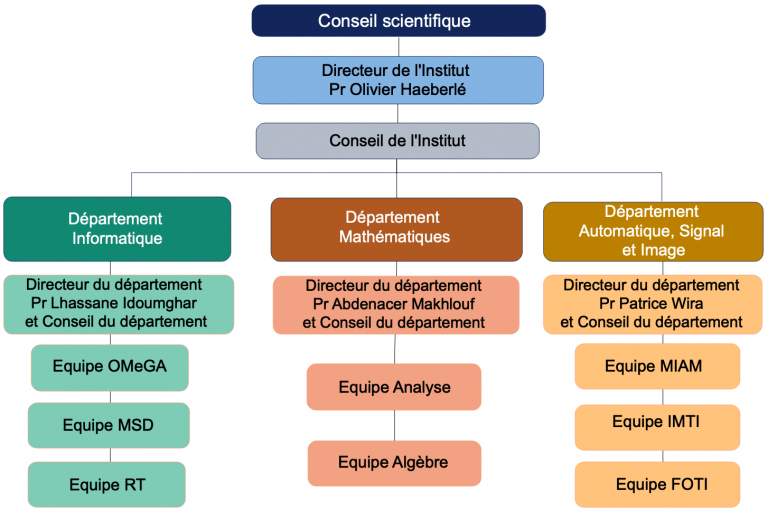
\includegraphics[width=1\textwidth]{irimas_organigramme}%
						\caption{Organigramme de l'\acrshort{IRIMAS}~\cite{IRIMAS_Organigramme}}%
						\label{fig:irimas_organigramme}%
					\end{figure}
				\paragraph*{}
					La répartition ainsi que les directeurs de ces départements sont visibles sur la figure \ref{fig:irimas_organigramme}. Durant le stage j'ai rejoint l'équipe \gls{OMeGA} du département informatique.
			\subsection{Équipe \acrshort{OMeGA}}
				\paragraph*{}
					Au sein du département informatique, l'équipe \gls{RTe} est situé à Colmar tandis que les équipe \gls{OMeGA} et \gls{MSD} sont actuellement hébergées dans l'aile sud du bâtiment Lumière de l'\gls{ENSISA} sur le campus Illberg à Mulhouse (point I sur le plan de l'annexe \ref{sec:uha_illberg_map}).
				\paragraph*{}
					L'équipe est sous la responsabilité de Lhassane Idoumghar (qui dirige aussi le département informatique) et est composée d'une douzaine de chercheurs et enseignants-chercheurs et de 5 doctorants qui travaillent essentiellement sur les axes de recherche ``Optimisation par Métaheuristiques'' et ``Algorithmique et Modélisations''.
				\paragraph*{}
					Une métaheuristique est un ensemble de concepts pouvant être utilisés pour définir des méthodes heuristiques pouvant être appliquées à un large éventail de problèmes différents, souvent des problèmes d'optimisation difficile. En d'autres termes, une métaheuristique peut être considérée comme un cadre algorithmique général qui peut être appliqué à différents problèmes d'optimisation avec relativement peu de modifications pour les adapter à un problème spécifique.
				\paragraph*{}
					``Le premier groupe de travail s'intéresse à l'algorithmique pour l'intelligence artificielle en développant de nouveaux algorithmes hybrides (basés sur des métaheuristiques à base d'agents intégrant des méthodes d'apprentissage) pour résoudre des problèmes d'optimisation mono-objectif ou multi-objectif de natures continues, discrètes et combinatoires, avec la prise en compte de l'aspect dynamique dans certains cas. L'adaptation et l'implémentation de ces futurs algorithmes hybrides sur des clusters hétérogènes de machines GPU sont également étudiées.''~\cite{IRIMAS_OMeGA}
				\paragraph*{}
					``L'activité du second groupe s'inscrit dans le thème d'analyse de données visuelles et géométriques (images, vidéo, nuages de points, courbes, etc.). Dans le cadre de cette thématique, ils développent des algorithmes et des concepts pour résoudre des problèmes de nature géométrique qui apparaissent dans de nombreuses disciplines de l'informatique [\ldots] ainsi que des techniques d'extraction d'information dans des données visuelles pour répondre à des problématiques de visualisation et d'analyses de scènes.''~\cite{IRIMAS_OMeGA}
				\paragraph*{}
					Laurent Moalic, qui a proposé le sujet de ce stage (détaillé dans la partie \ref{sec:presentation_stage}), est membre de l'équipe \gls{OMeGA}, le sujet proposé, ainsi que ces travaux en général, s'inscrivent dans l'axe Optimisation par Métaheuristiques du laboratoire.
	\chapter{Présentation du stage}\label{sec:presentation_stage}
		\section{Contexte du stage}
			\subsection{\acrshort{HEAD}}
				\paragraph*{}
					En \citeyear{Moalic2018} a été publié l'article \citetitle{Moalic2018}~\cite{Moalic2018} par \citeauthor{Moalic2018}, cet article propose l'utilisation de méthodes d'optimisation métaheuristiques hybrides sur le \gls{GVCP}.
				\paragraph*{}
					La coloration des sommets d'un graphe implique l'attribution d'une couleur à chaque sommet, de sorte que deux sommets adjacents (reliés par une arête) aient des couleurs différentes. Le \gls{GVCP} consiste à trouver le nombre minimal de couleurs, appelé nombre chromatique, requis pour colorer le graphe tout en respectant ces contraintes. La figure~\ref{fig:Petersen_graph_3-coloring} montre un exemple de solution a ce problème pour un graphe simple.
					\begin{figure}[H]
						\centering%
						
\includegraphics[width=0.25\textwidth]{Petersen_graph_3-coloring}%
						\caption{Une solution optimale au \acrshort{GVCP} pour le graphe de Petersen en utilisant 3 couleurs~\cite{wiki:Graphe_de_Petersen}}%
						\label{fig:Petersen_graph_3-coloring}%
					\end{figure}
				\paragraph*{}
					L'hybridation utilisée dans l'article pour résoudre ce problème est de type mémétique, c'est-à-dire qu'elle résulte de l'hybridation entre un algorithme génétique et un algorithme de recherche locale.
				\paragraph*{}
					Les algorithmes génétiques sont des métaheuristiques inspirées du processus de sélection naturelle qui appartiennent à la classe plus large des algorithmes évolutifs. Les algorithmes génétiques sont couramment utilisés pour générer des solutions de haute qualité aux problèmes d'optimisation et de recherche en s'appuyant sur des opérateurs inspirés de la biologie telles que la mutation, le croisement et la sélection.
				\paragraph*{}
					Les recherches locales prennent une solution potentielle à un problème et regardent ses voisins (c'est-à-dire des solutions similaires à l'exception de détails mineurs) dans l'espoir de trouver une solution améliorée. Les méthodes de recherche locales ont tendance à rester bloquées dans des régions sous-optimales ou sur des plateaux où de nombreuses solutions s'apparentent.
				\paragraph*{}
					L'algorithme proposé, \gls{HEAD}, est basé sur \gls{HEA}~\cite{Galinier1999} et fonctionne avec une population de deux individus. De plus il intègre une nouvelle façon de gérer la diversité a la population avec des solutions ``élites''. L'hybridation est faite avec une \gls{RT} adapté au \gls{GVCP}.
				\paragraph*{}
					Les \gls{RT} sont des métaheuristiques utilisant des méthodes de recherche locales en assouplissant leur règle de base. À chaque étape, des mouvements de détérioration peuvent être acceptés si aucun mouvement d'amélioration n'est disponible (comme lorsque la recherche est bloquée dans un minimum local). De plus, des interdictions (désignées par le terme tabou) sont introduites pour décourager la recherche de revenir à des solutions précédemment consultées.
				\paragraph*{}
					Les expériences menées sur un ensemble d'instance \gls{GVCP} difficiles du \gls{DIMACS}, montrent que \gls{HEAD} produit de bon résultats. Les résultats obtenus par \gls{HEAD} laissent penser que ce type d'approche pourrait être appliqué avec succès à d'autres problèmes \acrshort{NP}-complets.
				\paragraph*{}
					Les problèmes \acrshort{NP}-complets représentent les problèmes les plus difficiles de \acrfull{NP} qui est une classe de complexité utilisée pour classifier les problèmes de décision. \acrshort{NP} est l'ensemble des problèmes de décision pour lesquels chaque entrée du problème doit être associée à un ensemble de solutions de longueur polynomiale, dont la validité peut être testée rapidement (en temps polynomial).
				\paragraph*{}
					Si un problème \acrshort{NP}-complet a un algorithme en temps polynomial, tous les problèmes de \acrshort{NP} en ont. Bien qu'une solution à un problème \acrshort{NP}-complet puisse être vérifiée en temps polynomial, il n'existe aucun moyen connu de trouver une solution en temps polynomial. C'est-à-dire que le temps requis pour résoudre le problème en utilisant n'importe quel algorithme connu augmente exponentiellement avec la taille du problème. Les problèmes \acrshort{NP}-complets donc sont souvent traités en utilisant des méthodes heuristiques et des algorithmes d'approximation.
			\subsection{\acrshort{SCP} et \acrshort{USCP}}\label{sec:SCP_et_USCP}
				\paragraph*{}
					Le \gls{SCP}, fait partit des 21 problèmes \acrshort{NP}-complets de \citeauthor{Karp1972}~\cite{Karp1972}, il peut être énoncé comme suit:
				\paragraph*{}
					Étant donné un ensemble univers \(U = \{u_1, u_2, u_3, \dots, u_m\}\) et une famille \(S = \{s_1, s_2, \dots, s_n\}\) de sous-ensembles de \(U\) avec \(c_i\), coût du sous-ensemble \(s_i\), le problème consiste à trouver une sous-famille de \(S\) permettant de couvrir chaque élément de \(U\) au moins une fois avec un coût minimum. Un élément \(e\) de \(U\) est couvert par un sous-ensemble \(A\) si \(e \in A\).
				\paragraph*{}
					Dans le cas où tous les sous-ensembles \(s_i\) ont un coût identique, le problème est alors appelé \gls{USCP} ou \gls{UwSCP}, un exemple graphique d'instance d'\gls{USCP} est visible sur la figure \ref{fig:uscp_example}.
				\begin{figure}[H]
					\centering%
					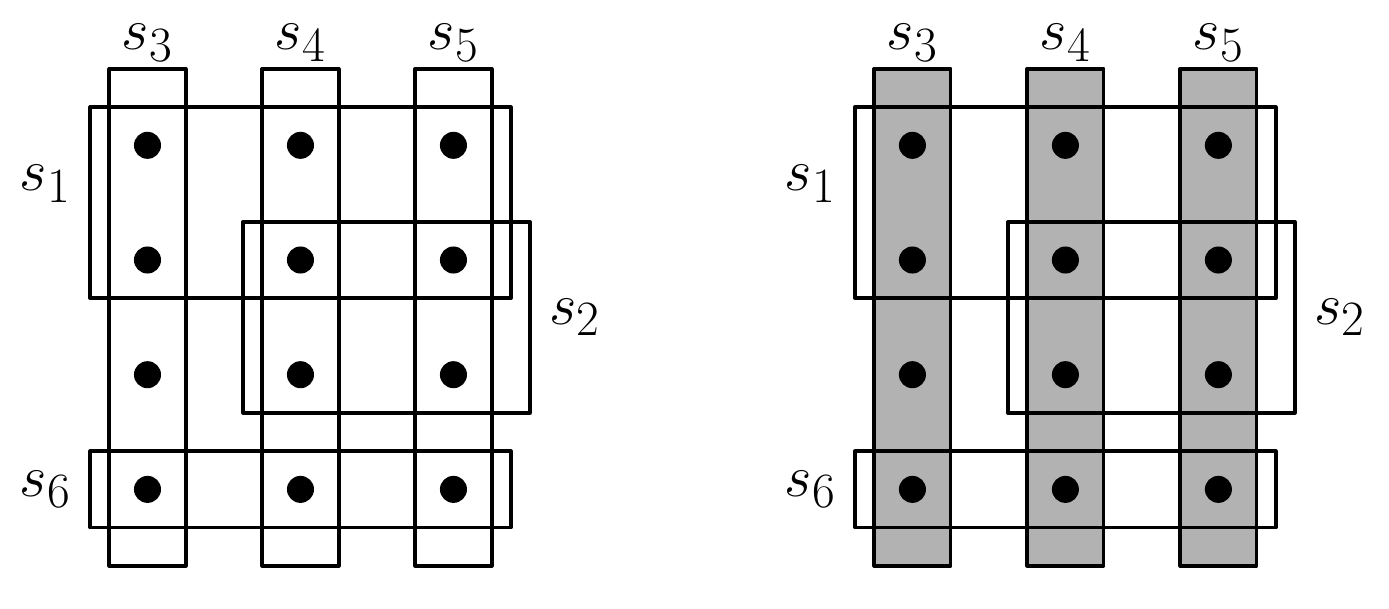
\includegraphics[width=0.65\linewidth]{uscp_example}%
					\caption{Exemple d'instance du \acrshort{USCP} et solution optimale (ensembles grisés)~\cite{Mount2017}}%
					\label{fig:uscp_example}%
				\end{figure}
				\paragraph*{}
					En général les instances de \gls{SCP} sont définies par une matrice d'incidence \(A = \left(a_{i,j}\right)\) de taille \(m \times n\) avec
					\[\forall i \in \{1,\ldots,m\},\ \forall j \in \{1,\ldots,n\},\ a_{i,j} = \left\{
						\begin{array}{ll}
							1 & \text{si } u_i \in s_j \\
							0 & \text{sinon}
						\end{array}
					\right.\]
					\(a_{i,j} = 1\) signifiant donc que le point \(u_i\) est couvert par le sous-ensemble \(s_j\), ainsi qu'un vecteur coût \(n\)-dimensionnel \(c = \left(c_j\right)\) avec \(\forall j \in N\), \(c_j\) le coût du sous-ensemble \(j\).
				\paragraph*{}
					Les solutions sont quant à elles définies par un vecteur \(n\)-dimensionnel \(x = \left(x_j\right)\) avec
					\[\forall j \in \{1,\ldots,n\},\ x_j = \left\{
						\begin{array}{ll}
							1 & \text{si } u_i \text{ fait parti de la solution}\\
							0 & \text{sinon}
						\end{array}
					\right.\]
					le coût de la solution étant égal à
					\[\sum_{j \in \{1,\ldots,n\}}{c_j x_j}\]
					et la solution étant valide si
					\[\forall i \in \{1,\ldots,m\}\ ,\sum_{j \in \{1,\ldots,n\}}{a_{ij}x_j} \ge 1\]
				\paragraph*{}
					Par exemple, l'instance suivante, définie par la matrice d'incidence \(A\) et le vecteur coût \(c\) a comme solution optimale le vecteur \(x\):
					\[
					\begin{blockarray}{ccccccccc}
						& s_1 & s_2 & s_3 & s_4 & s_5 & s_6 & s_7\\
						\begin{block}{c(ccccccc)c}
							    & 0 & 1 & 1 & 0 & 0 & 0 & 1 & u_1\\
							    & 0 & 0 & 1 & 0 & 1 & 1 & 0 & u_2\\
							A = & 1 & 1 & 0 & 1 & 0 & 1 & 0 & u_3\\
							    & 0 & 0 & 0 & 0 & 1 & 1 & 1 & u_3\\
							    & 1 & 0 & 1 & 0 & 0 & 0 & 1 & u_4\\
						\end{block}
						\\
						\begin{block}{c(ccccccc)c}
							c = & 3 & 1 & 2 & 4 & 1 & 2 & 1 &\\
						\end{block}
						\\
						\begin{block}{c(ccccccc)c}
							x = & 0 & 1 & 1 & 0 & 0 & 0 & 1 &\\
						\end{block}
					\end{blockarray}
					\]
				\paragraph*{}
					Il est à noté que, bien que le \gls{USCP} soit un cas particulier du \gls{SCP}, du fait de l'information réduite de par l'absence de poids pour les sous-ensembles, il est généralement considéré que le \gls{USCP} est plus difficile à résoudre que le \gls{SCP}~\cite{Yelbay2015}.
		\section{Objectifs du stage}
			\subsection{Objectif initial}
				\paragraph*{}
					L'objectif du stage est de développer des algorithmes hybrides avec une recherche poussée de performance pour le \gls{USCP}, la piste première à explorer étant d'utiliser les principes de \gls{HEAD} et de les adapter au \gls{USCP}.
				\paragraph*{}
					Le développement d'algorithmes méthaheuristique se faisant en se basant sur les travaux existant, il sera nécessaire d'analyser la littérature du problème afin d'identifier les recherches locales, opérateur de sélection, opérateurs de croisement et mutation efficaces pour le problème afin de les comparer et de sélectionner les plus adaptés pour notre algorithme.
				\paragraph*{}
					Pour réaliser ces comparaison et afin d'évaluer la performance de notre algorithme, il sera nécessaire d'identifier les instances de benchmark classiques de la littérature ainsi que les résultats obtenus par les méthodes les plus efficaces connues afin de ce comparer à ces dernières.
				\paragraph*{}
					Une fois toutes ces recherches réalisées, le développement pourra commencer, dans un premier temps il faudra implémenter les structures et algorithmes de base lié au \gls{SCP}, puis il faudra implémenter la recherche locale que nous utiliserons dans notre hybridation et enfin implémenter l'algorithme en lui même.
				\paragraph*{}
					Après cela viendra la phase de réglage ou il faudra alterner entre benchmarks, optimisation logicielle et variation des paramètres et composants de l'algorithme afin optimiser son efficacité. Une fois les réglages terminé, une étude comparative de la performance de l'algorithme sera réalisé.
			\subsection{Objectifs supplémentaires}
				\paragraph*{}
					Après que la première version notre algorithme ai été conçut et implémenté (voir section \ref{sec:memetic_algorithm} pour le détail des différentes versions de l'algorithme), nous avons commencé à obtenir de bon résultats, il a donc été décidé de soumettre à la conférence \acrshort{ROADEF2020} qui est le ``\acrlong{ROADEF2020}''~\cite{ROADEF2020}.
				\paragraph*{}
					La deuxième version de l'algorithme a été développé et a servit pour la publication pour \acrshort{ROADEF2020}, les résultats de cette nouvelle version étant encore meilleurs et apportant une contribution assez significative, il a été décidé de soumettre à la conférence \acrshort{LION14} qui est la ``\acrlong{LION14}''~\cite{LION14}.
				\paragraph*{}
					Enfin, le dernier objectif qui fut ajouté est d'utiliser l'algorithme développé au cours du stage afin de résoudre des instances de \gls{GVCP} à partir de solutions sous-optimales qui sont générées de façon très rapide par l'algorithme de Laurent.
				\paragraph*{}
					Ces nouveaux objectif ayant été ajouté durant le stage (voir section \ref{sec:planning} pour les dates), ils nécessitent de déjà connaitre ce qui à été réalisé durant le stage avant leur ajout, ils seront donc explicité plus en détail avec le travail réalisé durant le stage dans la section \ref{sec:work}.
		\section{Organisation du stage}
			\subsection{Environnement de travail}
				\paragraph*{}
					Un bureau avec poste informatique, proche des autres membres de l'équipe, m'a été attribué, il est partagé avec Dominique Schmitt, enseignant-chercheur sur l'axe Algorithmique et Modélisations de l'équipe \gls{OMeGA}. Dans la même zone du bâtiment se trouve les bureaux de Laurent Moalic, Mathieu Brévilliers et Julien Lepagnot avec qui j'ai le plus travaillé sur la partie recherche du stage.
				\paragraph*{}
					La nature du stage le permettant (pas de problèmes de confidentialité), j'ai décider de travailler sur mon ordinateur personnel, ce dernier est assez bien équipé pour développer et tester en local le \solver{} (programme ou sera implémenter les différents algorithmes de résolution). Il est équipé d'un Intel Core i7-4710MQ (Quad-Core 2.5 GHz / 3.5 GHz Turbo - cache 6 Mo) avec 16 Go de mémoire vive DDR3L. Le \solver{} développé n'utilise pas le GPU et ne nécessite que peut d'espace disque.
				\paragraph*{}
					Les programmes ont majoritairement été développé sur Linux, plus précisément la distribution Debian unstable (connu aussi sous le nom de code Sid), qui est très adapté au développement logiciel car renfermant les paquets les plus récents qui viennent d'être introduits dans le système Debian (voir annexe \ref{sec:programs_versions} pour les versions des différents programmes utilisés).
				\paragraph*{}
					Le programmes ont été développés en \Cpp{}17\footnote{Révision de 2017 du \href{https://www.iso.org/standard/68564.html}{standard ISO/IEC 14882}}, conçu pour fonctionner sur Linux et Windows et pour embarquer toutes leur dépendances afin d'être autonome. Ils utilisent \textit{CMake} comme build-system et \textit{Make} ou \textit{Ninja} comme sous-système et sont compilables en utilisant \textit{gcc} et \textit{clang} sous Linux et \textit{Microsoft Visual \Cpp{} compiler} sous Windows. Le support de plusieurs plateformes d'exécution et compilateurs n'était pas nécessaire pour ce projet mais facilement atteignable, j'ai donc décidé de le prendre en compte pour que mon travail soit le plus facile possible à utiliser et reprendre.
				\paragraph*{}
					Le développement c'est fait sur Linux en utilisant l'\gls{IDE} \textit{CLion} tandis que la vérification de la compilation et compatibilité Windows c'est fait avec l'\gls{IDE} \textit{Microsoft Visual Studio}. La rédaction des différent scripts de lancement des benchmarks ont été rédigés avec l'éditeur \textit{Sublime Text}.
				\paragraph*{}
					Le code du projet est formaté en utilisant \textit{clang-format} avec un style personnalisé et est fréquemment analysé avec l'analyseur statique \textit{clang-tidy} afin d'éviter au maximum les erreurs de code du à une inattention ou une faute de frappe.
				\paragraph*{}
					Le code, les données et les documents du projet ont été versionné avec \textit{git} dans 4 dépôts:
					\begin{description}
						\item[USCP] contient le code et les ressources des différent programmes développés
						\item[USCP\_instances] contient les instances de benchmark utilisées ainsi que de la documentation sur ces dernières
						\item[USCP\_results] contient les résultats des différent benchmarks réalisés ainsi que de la documentation sur ces derniers
						\item[UTBM\_ST50\_Rapport\_de\_stage\_IRIMAS] contient les rapport et présentations demandées par l'\gls{UTBM} et l'\gls{UQAC}, notamment les rapports de stage
					\end{description}
					Chacun de ses dépôt a pour \textit{remote} un dépôt GitHub privé afin de toujours avoir une sauvegarde en cas d'accident.
			\subsection{Cluster \acrshort{HPC}}
				\paragraph*{}
					Le méso-centre de l'Université de Strasbourg se situe parmi les 4 centres de calcul régionaux les plus puissants en France. Il est opéré par le pôle \gls{HPC} de la Direction du numérique de l'Université de Strasbourg~\cite{UNISTRA_Calcul_scientifique}. Au cours de la 6\textsuperscript{ème} semaine du stage j'ai obtenu l'accès à la partition ``public'' au cluster \gls{HPC} du service de calcul scientifique du méso-centre de Strasbourg.
				\paragraph*{}
					Les ressources de calcul du \gls{HPC} auquel j'ai eu accès sont composées de 1.3Po (1\,266\,700Go) de stockage, 9\,968 cœurs de calcul, environ 47To (47\,818Go) de mémoire vive, le tout réparti sur 467 nœuds de calcul. Parmi les nœuds, on compte notamment:
					\begin{itemize}
						\item 56 noeuds Intel Xeon Nehalem/Westmere à 24Go de RAM, financés par mutualisation
						\item 145 noeuds Intel Xeon Sandy-Bridge à 16 coeurs et 64Go de RAM, financés par l'\gls{Equip@meso} avec le soutien du conseil scientifique de l'Université de Strasbourg
						\item 150 noeuds Intel Sandy et Ivy Bridge, Westmere de 16 ou 24 cœurs et de 64 à 128Go de RAM, financés par mutualisation
					\end{itemize}
					Tous les processeurs sont d'architecture x86\_64, et les nœuds de login et de calculs utilisent \textit{Scientific Linux} 7.5\footnote{Équivalent RedHat même version, voir \url{http://www.scientificlinux.org/}}.
				\paragraph*{}
					Le cluster \gls{HPC} a servit à réaliser l'ensemble des benchmarks du projet, ces benchmarks demandant énormément d'heures de calcul (voir sec \ref{sec:analyse_stage_travail}), il n'aurais pas été possible d'avoir des données aussi conséquentes sur lesquelles travailler sans cet accès au méso-centre.
				\paragraph*{}
					Après que l'équipe en charge du méso-centre ai installé notre clé ssh sur le noeud de login, l'accès au cluster \gls{HPC} se fait en ssh. L'utilisation des noeuds de calcul se fait par l'intermédiaire de \textit{Slurm Workload Manager} qui gère les différent noeuds, partitions de calcul, groupes d'utilisateurs, \ldots{} et gère la répartitions des taches (appelées job) par un système de priorités et de files d'attentes.
				\paragraph*{}
					Différents programmes sont mis a disposition sur le cluster par l'intermédiaire de \textit{GNU Modules} qui permet de les charger. Les deux modules utilisé durant le stage sont \texttt{cmake/cmake-3.12.2} et \texttt{gcc/gcc-9} pour la compilation des programmes.
				\paragraph*{}
					Le code des programmes développés est récupéré sur le cluster avec \textit{git} par l'intermédiaire des dépôts privés sur Github tandis que les résultats de l'exécution du \solver{} pour les différents benchmarks sont téléchargés du cluster avec \textit{rsync}.
			\subsection{Déroulement du stage}\label{sec:planning}
				\begin{landscape}
					\begin{figure}[H]
						\centering%
						\hspace*{-0.5cm}
						\resizebox{1.1\paperwidth}{!}{\import{../figures/}{planning.tex}}%
						\caption{Planning détaillé du stage}%
						\label{fig:planning}%
					\end{figure}
				\end{landscape}
				\paragraph*{}
					Le déroulement général du stage est visible sur la figure \ref{fig:planning} qui représente les grandes périodes du stage, les évènements importants qui ont influencé le stage et la répartition de mon temps entre les activités principales:
					\begin{itemize}
						\item La lecture d'articles scientifique et de documentation: la review de la littérature initiale, la documentation des librairies utilisées pour le développement des programmes, la documentation pour l'utilisation du cluster \gls{HPC},\ldots
						\item La programmation du \solver{}: les éléments de base lié au \gls{USCP}, le parsage et la réduction des instances, l'algorithme \gls{RWLS}, l'algorithme Mémétique\ldots
						\item La programmation du \printer{}: la lecture des données générées par le \solver{}, la traitement des données, la réalisation de statistiques, la génération de tables et de documents,\ldots
						\item La rédaction: documentation pour les programmes et les instances et les benchmark, les différentes soumissions aux conférences,\ldots
					\end{itemize}
				\paragraph*{}
					Le stage a commencé par une review de la littérature (détaillée dans la section \ref{sec:review_litterature}) en partant d'articles déjà repérés par Matthieu et de l'article \citetitle{Kritter2019} de \citeauthor{Kritter2019} publié en \citeyear{Kritter2019}, le \gls{OCP} dont traite l'article se réduisant au \gls{USCP}, l'article passe en revu toutes les méthodes efficaces pour résoudre le \gls{SCP} et le \gls{USCP}.
				\paragraph*{}
					Cette review de la littérature mena, au cours de la 2\textsuperscript{ème} semaine de stage, au choix de \gls{RWLS} comme recherche locale pour notre algorithme mémétique. Après la première implémentation de \gls{RWLS} (voir section \ref{sec:impl_RWLS}) et ma demande d'accès au cluster \gls{HPC}, au cours de la 6\textsuperscript{ème} semaine de stage, j'ai décider de séparer le code en 3 cibles (1 librairie et 2 programmes):
					\begin{itemize}
						\item \common{}: Librairie qui contient les structures de données nécessaire à la manipulation, la lecture et l'écriture des instances du \gls{USCP}, contient aussi les informations relatives aux instances de banchmark classique du \gls{USCP} ainsi que des fonctions et classes utilitaires (formatage, logging,\ldots)
						\item \solver{}: Programme en ligne de commande pour la résolution du \gls{USCP}, il implémente différentes méthodes de résolution (greedy, \gls{RWLS}, algorithme Mémétique). Il prend en entrée les instances à résoudre, les méthodes à utiliser et les paramètres de ces méthodes. Il génère des rapports d'exécution contenant les informations relative aux résolutions réalisées (solution trouvée, durée et étapes de résolution effectué au moment ou la solution a été trouvée,\ldots)
						\item \printer{}: Programme en ligne de commande pour le traitement des rapports d'exécution du \solver{}, il prend en entrée les dossiers/fichiers contenant les rapports d'exécution et génère des documents \LaTeX{} contenant des tables présentant les résultats obtenus par chaque méthode de résolution par instance, des statistiques sur les résultats obtenus, des comparaison des résultats d'une même méthode avec différent paramètres,\ldots
					\end{itemize}
				\paragraph*{}
					Toujours durant la 6\textsuperscript{ème} semaine j'ai obtenu l'accès au méso-centre, je me suis donc renseigné sur l'utilisation de ce dernier et j'ai commencé à banchmarker mon implémentation de \gls{RWLS} sur le cluster \gls{HPC}. Jusqu'à la 8\textsuperscript{ème} semaine j'ai travaillé sur mon implémentation de \gls{RWLS} pour être strictement conforme à sa description dans~\cite{Gao2015}. En parallèle j'ai développé le \printer{} en fonction des besoins de traitement des benchmarks réalisés.
				\paragraph*{}
					Durant la 9\textsuperscript{ème} semaine du stage à eu lieu la conférence \acrshort{EA2019} qui est la ``\acrlong{EA2019}''~\cite{EA2019}. La conférence a eu lieu dans les locaux de la \gls{FST}, sur le site de l'\gls{UHA}, les 29 et 30 octobre 2019. J'ai assisté à la conférence les deux jours et ce fut très intéressant.
				\paragraph*{}
					À la 10\textsuperscript{ème} semaine du stage j'ai commencé la conception et l'implémentation de l'algorithme Mémétique (voir section \ref{sec:memetic_algorithm}), en parallèle de cela je réalisait des benchmarks, sur le cluster \gls{HPC}, des différentes évolutions de l'algorithme. La 1\textsuperscript{ère} version de ce dernier a rapidement donné de bon résultats et amélioré une \gls{BKS}, à la 11\textsuperscript{ème} semaine il été décidé de soumettre à la conférence \acrshort{ROADEF2020}.
				\paragraph*{}
					Au cours de la 12\textsuperscript{ème} semaine j'ai rédigé la majorité de la soumission et j'ai implémenté la 2\textsuperscript{ème} version de l'algorithme qui ajoute le croisement des poids. Les résultats du benchmark de cette deuxième version étant meilleurs et améliorant encore d'autres \gls{BKS}, c'est cette version de l'algorithme qui a été présenté dans la soumission \acrshort{ROADEF2020} qui à été déposé au cours de la 13\textsuperscript{ème} semaine.
				\paragraph*{}
					À partir de la 14\textsuperscript{ème} semaine j'ai commencé à essayer différentes idées de modifications de l'algorithme Mémétique ainsi que différent opérateurs de croisement des solutions et des poids de \gls{RWLS}. Durant la 15\textsuperscript{ème} semaine j'identifie que le nombre d'étapes de \gls{RWLS} le plus efficace pour notre algorithme diffère énormément entre les instances et j'introduis le système d'évolution dynamique du nombre d'étapes de \gls{RWLS}.
				\paragraph*{}
					La 3\textsuperscript{ème} version de l'algorithme étant très performante et améliorant 6 \gls{BKS}, durant le 16\textsuperscript{ème} semaine il a été décider de soumettre a la conférence \acrshort{LION14}. Le site de l'\gls{UHA} est fermé durant la 17\textsuperscript{ème} et 18\textsuperscript{ème} semaines pour les vacances de fin d'année, durant ces vacances je rédige la première version de la soumission pour \acrshort{LION14}.
				\paragraph*{}
					A la rentrée, durant la 19\textsuperscript{ème} et 20\textsuperscript{ème}, je finis d'implémenter et de tester le système d'évolution dynamique du nombre d'étapes de \gls{RWLS} et j'optimise la réduction des instances mais je ne peut pas réaliser de benchmark car le cluster \gls{HPC} est hors service à cause du déménagement du méso-centre. J'applique les modifications demandé par les reviewer pour la soumission de \acrshort{ROADEF2020} et j'améliore la soumission pour \acrshort{LION14}.
				\paragraph*{}
					Durant la 21\textsuperscript{ème} semaine, je règle les derniers détails de l'algorithme Mémétique et je réalise plusieurs optimisations afin de pouvoir réaliser un benchmark de l'algorithme Mémétique sur les instances \instance{RAIL} avec un paramètre de durée raisonnable.
				\paragraph*{}
					Durant la 22\textsuperscript{ème} semaine, Matthieu et Laurent reprennent la soumission de \acrshort{LION14}, l'améliorent et me demandent de faire des modifications dans les schémas et algorithmes, je réalise aussi les derniers benchmarks pour les tableaux de résultats de la version finale de l'article. Les résultats soumis améliorent 8 \gls{BKS} et apportent une \gls{BKS} à une instance (\instance{STS2187}) encore non traitée dans la littérature. J'implémente aussi le support des instances issues du \gls{GVCP}, je benchmark l'algorithme sur des instances générées à partir de solutions du \gls{GVCP} données par Laurent. Je réalise des statistiques d'utilisation de \textit{git} et du cluster \gls{HPC} pour en faire des figures pour les rapports de stage.
				\paragraph*{}
					La 23\textsuperscript{ème}, et dernière, semaine du stage est dédié à la rédaction des différents rapports demandés par l'\gls{UTBM} et l'\gls{UQAC} ainsi que la réalisation de benchmarks finaux de la dernière version du \solver{}.
	\chapter{Travail réalisé}\label{sec:work}
		\section{Review de la littérature}\label{sec:review_litterature}
			\subsection{État de l'art}
				\paragraph*{}
					La première étape du stage a été de réaliser un état de l'art, pour cela j'ai analysé la littérature en lien avec le \gls{USCP} en partant de l'article \citetitle{Kritter2019}, écrit par des membres du laboratoire et un ensembles d'articles déjà repérés par Matthieu. Parmi ces articles, certains présentent des recherches locales, afin d'en sélectionner une pour l'hybridation de notre algorithme Mémétique, certains présentent des algorithmes génétiques, afin de repérer les différent opérateurs de croisement efficaces pour le \gls{USCP} et le dernier présente des procédures de réduction.
				\paragraph*{\citetitle{Kritter2019} de \citeauthor{Kritter2019} (\citeyear{Kritter2019})~\cite{Kritter2019}\\}
					Cet article est une review de la littérature très complète sur le \gls{OCP} ainsi que sur le \gls{SCP} et le \gls{USCP}. Il reprend la majorité des approches utilisées sur le \gls{SCP}, regroupe tout les résultats obtenus par les auteurs de ces différent algorithmes et identifie les plus efficaces. Il indique ainsi que l'approche la plus efficace pour le \gls{USCP} est à ce jour l'algorithme \gls{RWLS} proposé par \citeauthor{Gao2015} en \citeyear{Gao2015}~\cite{Gao2015}, ce dernier atteignant ou améliorant les \gls{BKS} de toutes les instances de benchmark classiques hors \instance{RAIL} à l'exception des instances \instance{C.1-4} pour lesquelles l'algorithme de \citeauthor{Akhter2015}~\cite{Akhter2015} trouve des résultats étonnamment meilleurs jamais atteint par personne d'autre. Les instances \instance{C.1-4} étant très simples a résoudre je pense personnellement a une erreur de la part de \citeauthor{Akhter2015} mais je ne peut pas en être sur.\\
					L'article donne les références pour l'algorithme greedy pondéré classique~\cite{Chvatal1979}, pour la réduction des instances~\cite{Beasley1987}, pour de nombreux algorithmes génétiques (voir articles suivants). Il présente toutes les instances de benchmark classiques, leur caractéristiques et leurs \gls{BKS}.
				\paragraph*{\citetitle{Gao2015} de \citeauthor{Gao2015} (\citeyear{Gao2015})~\cite{Gao2015}\\}
					Cet article présente l'algorithme \acrfull{RWLS} qui est une heuristique pour le \gls{USCP} qui réunit 3 composant dans une recherche locale:
					\begin{itemize}
						\item un schéma de pondération, qui met à jour les poids des éléments non couverts pour empêcher la convergence vers les optima locaux
						\item des stratégies tabou pour éviter les cycles pendant la recherche
						\item une méthode d'horodatage pour résoudre les égalités lors de la hiérarchisation des ensembles
					\end{itemize}
					\gls{RWLS} améliore 14 \gls{BKS} sur les instances de benchmark classiques, c'est l'algorithme que nous avons utilisé comme recherche locale, il est détaillé dans la section \ref{sec:RWLS}.
				\paragraph*{\citetitle{Musliu2006} de \citeauthor{Musliu2006} (\citeyear{Musliu2006})~\cite{Musliu2006}\\}
					Cet article présente une recherche locale qui partage plusieurs idées avec \gls{RWLS}, notamment un cycle de ajout/retrait de sous-ensemble à une solution invalide composée de 1 colonne de moins que la meilleure solution valide rencontrée ainsi qu'une stratégie tabou. C'est le concurrent principal de \gls{RWLS}, il est le principal algorithme de comparaison dans \cite{Gao2015} et est égalé ou surpassé par \gls{RWLS} pour toutes les instances non-\instance{RAIL}.
				\paragraph*{\citetitle{Beasley1996} de \citeauthor{Beasley1996} (\citeyear{Beasley1996})~\cite{Beasley1996}\\}
					Cet article présente un algorithme génétique pour le \gls{SCP}, cet algorithme utilise une représentation binaire telle que présenté dans la section \ref{sec:SCP_et_USCP} avec le vecteur \(x\) car plus performante qu'une représentation numérique avec une liste des sous-ensembles sélectionnés. La sélection des parents se fait par tournois binaire, le croisement se fait en prenant des sous-ensembles des parent en fonction de leur fitness puis réparant la solution générée, la mutation se fait en ajoutant ou supprimant aléatoirement un sous-ensemble puis réparant la solution.
				\paragraph*{\citetitle{Eremeev1999} de \citeauthor{Eremeev1999} (\citeyear{Eremeev1999})~\cite{Eremeev1999}\\}
					Cet article présente un algorithme génétique pour le \gls{SCP}, cet algorithme, contrairement a la majorité des algorithmes génétiques proposés pour le \gls{SCP} n'utilise une représentation binaire. Cet représentation requiert une opération supplémentaire de suppression des sous-ensembles redondants après l'application de l'opérateur de croisement. La sélection des parents se fait par roulette sur les rangs, le croisement se fait avec la résolution du sous-problème composé uniquement des sous-ensembles des parent avec la méthode du simplex dual, la mutation se fait en choisissant un sous-ensemble alternatif pour chaque élément.
				\paragraph*{\citetitle{Aickelin2002} de \citeauthor{Aickelin2002} (\citeyear{Aickelin2002})~\cite{Aickelin2002}\\}
					Cet article présente un algorithme génétique ``indirecte'' pour le \gls{SCP}, l'algorithme est dit indirecte car il utilise un procédure de décodage pour transformer un ordonnancement des sous-ensembles en une solution. La population n'est donc pas composé de solutions au problème mais d'ordonnancement des sous-ensembles qui sont décodés et évalués pour obtenir leur fitness. La sélection des parents se fait par roulette sur les rangs, le croisement se fait avec le \gls{PUX} avec \(P = 0.66\), la mutation se fait en inversant 2 sous-ensembles.
				\paragraph*{\citetitle{Kornilakis2002} de \citeauthor{Kornilakis2002} (\citeyear{Kornilakis2002})~\cite{Kornilakis2002}\\}
					Cet article présente un algorithme génétique pour résoudre le \gls{SCP} avec une application au problèmes d'assignation d'équipages. L'algorithme utilise une représentation binaire, la sélection des parents se fait par roulette sur les rangs, le croisement se fait avec le \gls{UX} et une réparation, la mutation se fait en ajoutant ou supprimant un sous-ensemble en fonction de la densité de la meilleure solution puis réparant la solution.
				\paragraph*{\citetitle{Beasley1987} de \citeauthor{Beasley1987} (\citeyear{Beasley1987})~\cite{Beasley1987}\\}
					Cet article présente un algorithme pour résoudre le \gls{SCP} mais aussi plusieurs procédures de réduction pour les instances de \gls{SCP} facilement adaptables au \gls{USCP} dont les deux majeures sont \textit{column domination} et \textit{column inclusion}. Ces procédures seront détaillées dans la section \ref{sec:reduction}.
			\subsection{\acrshort{RWLS}}\label{sec:RWLS}
				\paragraph*{}
					\gls{RWLS} est la recherche locale choisie pour notre hybridation, c'est un algorithme heuristique qui repose principalement sur un schéma de pondération qui met à jour les poids des éléments non couverts pour empêcher la convergence vers les optima locaux. Le schéma de pondération guide l'algorithme en utilisant 2 concepts, le poids pour les éléments et le score pour les sous-ensembles.
				\paragraph*{}
					Le poids d'un élément représente la difficulté à couvrir cet élément, il est initialisé à 1 et augmenté de 1 pour chaque étape de l'algorithme ou l'élément laissé non couvert.
				\paragraph*{}
					Le score d'un sous-ensemble représente l'utilité du sous-ensemble dans la solution pour couvrir les éléments difficilement couvrables de l'instance. Si le sous-ensemble fait partie de la solution, son poids est l'opposé de la somme des poids des éléments qu'il est le seul à couvrir dans la solution. S'il ne fait pas partie de la solution, son poids est la somme des poids des éléments qu'il serait le seul à couvrir s'il était ajouté à la solution.
				\paragraph*{}
					Ainsi, les sous-ensembles qui font partie de la solution ont des scores négatifs, les sous-ensembles ne faisant pas partie de la solution ont des scores positifs et les sous-ensembles inutiles pour la solution ont des scores nuls. Ce qui signifie que le sous-ensemble inclut dans la solution avec le meilleur score est le moins utile a la solution et que le sous-ensemble non-inclut dans la solution avec le meilleur score serait le plus utile à ajouter à la solution.
				\paragraph*{}
					\gls{RWLS} commence par générer une solution greedy, puis fonctionne par étapes de manière itérative, les étapes peuvent se découper en sous-étapes comme suit:
					\begin{enumerate}[label=(\arabic*)]
						\item\customlabel{it:RWLS1}{(1)}\tikzremember{RWLS1}tant que la solution est valide:
							\begin{enumerate}[label=(\alph*)]
								\item\customlabel{it:RWLS1a}{(1.a)}\tikzremember{RWLS1a}enregistrer la solution comme la meilleure rencontrée jusqu'à présent
								\item\customlabel{it:RWLS1b}{(1.b)}\tikzremember{RWLS1b}\textbf{retirer} le sous-ensemble avec le meilleur score de la solution
							\end{enumerate}
						\item\customlabel{it:RWLS2}{(2)}\tikzremember{RWLS2}\textbf{retirer} le sous-ensemble avec le meilleur score de la solution
						\item\customlabel{it:RWLS3}{(3)}\tikzremember{RWLS3}sélectionner aléatoirement un élément non-couvert
						\item\customlabel{it:RWLS4}{(4)}\tikzremember{RWLS4}\textbf{ajouter} le sous-ensemble avec le meilleur score couvrant cet élément (les stratégies tabou empêchant de boucler)
						\item\customlabel{it:RWLS5}{(5)}\tikzremember{RWLS5}rendre le sous ensemble ajouté tabou et incrémenter le nombre d'étapes
					\end{enumerate}
					\begin{tikzpicture}[remember picture,overlay,x=1pt,y=1pt]
						\draw[->,>=Latex,dashed] ($(RWLS5)+(-25,0)$) -- ++(-12.5,0) |- ($(RWLS1)+(-25,0)$);
						\draw[->,>=Latex,dashed] ($(RWLS1b)+(-25,0)$) -| ($(RWLS1)+(-12.5,-7.5)$);
					\end{tikzpicture}
				\paragraph*{}
					\gls{RWLS} réalise cette boucle jusqu'à ce que la limite d'étapes soit atteinte, le nombre d'étapes est le seul critère d'arrêt mais il peut être remplacé par une limite de temps. \gls{RWLS} travaille avec une solution non valide qui compte 1 sous-ensemble de moins que la meilleure rencontrée, pour cela la sous-étape \ref{it:RWLS1} commence par retirer des sous-ensembles jusqu'à atteindre une solution non valide. Si la meilleure solution trouvée est composé de \(k\) sous-ensembles, alors \gls{RWLS} descendra à \(k - 1\) sous-ensembles avec la sous-étape \ref{it:RWLS1}, puis commencera à changer des sous-ensembles avec les sous-étapes \ref{it:RWLS2} et \ref{it:RWLS4} jusqu'à obtenir une solution valide a \(k - 1\) sous-ensembles qui deviendra la nouvelle meilleur solution en rebouclant sur la sous-étape \ref{it:RWLS1}. L'algorithme repose donc sur une alternance de 2 opérations, \textbf{retirer} aux sous-étapes \ref{it:RWLS1b} et \ref{it:RWLS2} et \textbf{ajouter} à la sous-étape \ref{it:RWLS4}.
				\paragraph*{}
					\gls{RWLS} utilise un concept de voisinage, dans \cite{Gao2015} il est définit que le voisinage d'un sous-ensemble est l'ensemble des sous-ensembles dont l'intersection de la couverture avec le sous-ensemble considéré n'est pas vide. Dit autrement, tous les sous-ensemble dont la couverture a 1 point ou plus en commun sont voisins.
				\paragraph*{}
					La première stratégie tabou de l'algorithme est mise en oeuvre avec un flag \textit{canAddToSolution} associé à chaque sous-ensemble qui indique si ce dernier peut être ajouté à la solution. Tout les flags sont initialisé à \textit{true}, l'opération \textbf{retirer} passe le flag du sous-ensemble retiré à \textit{false} et les 2 opération (\textbf{retirer} et \textbf{ajouter}) passent les flags de tout les voisins à \textit{true}. Ce système évite qu'un sous-ensemble soit retiré puis ajouté de nouveau juste après, un sous-ensemble retiré doit attendre l'ajout ou le retrait d'un de ses voisins pour pouvoir de nouveau être ajouté.
				\paragraph*{}
					La deuxième stratégie tabou de \gls{RWLS} est une liste \gls{FIFO} de taille 2 de sous-ensembles interdis, la sous-étape \ref{it:RWLS5} ajoute à la liste le sous-ensemble ajouté à la solution durant l'étape, en retirant d'abord un élément si la liste est pleine. La liste étant \gls{FIFO} de taille 2, chaque élément ajouté est interdit à la sélection pour l'opération \textbf{retirer} pendant 2 étapes.
				\paragraph*{}
					Les opérations \textbf{retirer} et \textbf{ajouter} doivent aussi mettre a jour le score de tout les sous-ensembles voisins du sous-ensemble ajouté ou retiré, car le score est lié à l'unicité de la couverture des points et changer les sous-ensembles composant la solution va inévitablement avoir des répercutions sur les scores des sous-ensembles. Comme dit précédemment, à chaque étape de \gls{RWLS} le poids des éléments non couverts augmente de 1, bien que cela ne soit pas présent dans les algorithmes de \cite{Gao2015}, il faut aussi mettre a jour le score de tout les sous-ensembles qui couvrent ces élément afin que leur score reste conforme a la définition du score.
				\paragraph*{}
					Cette exposition simplifiée du fonctionnement de \gls{RWLS} est incomplète par rapport à \cite{Gao2015} mais, je pense, suffisante pour aborder la suite de ce rapport et les explications du travail réalisé durant ce stage.
			\subsection{Instances de benchmark}
				\paragraph*{}
					Au total, 98 instances de benchmark sont été identifiées, 96 sont classiquement utilisées dans la littérature pour évaluer l'efficacité des méthodes de résolution du \gls{SCP} et du \gls{USCP} et 2 (\instance{STS1215} et \instance{STS2187}) sont moins utilisées, mais sont dans la continuité d'un set d'instances classiques. 87 de ces instances proviennent de OR-Library~\cite{Beasley1990b} et 11 des \gls{STS}~\cite{Fulkerson1974}. Pour traiter les instances pondérées comme instances de \gls{USCP}, il suffit d'ignorer les poids des colonnes de l'instance.
				\paragraph*{}
					La table~\ref{tab:instances_orlibrary_random} contient le détail des 70 instances de OR-Library générées aléatoirement\footnote{En utilisant le thème de \citeauthor{Balas1980}~\cite{Balas1980}}, les ensembles \instance{4} à \instance{6} proviennent de~\cite{Balas1980}, les ensembles \instance{A} à \instance{E} de~\cite{Beasley1987} et les ensembles \instance{NRE} à \instance{NRH} de~\cite{Beasley1990a}. Les optima de certaines de ces instances sont connus dans un contexte non-unicost mais pas lorsque traité en unicost, l'exception étant les instances de l'ensemble \instance{E} qui sont unicost mais triviales à résoudre.
				\begin{table}[H]
					\centering
					\caption{Ensembles d'instances aléatoires de OR-Library}
					\label{tab:instances_orlibrary_random}
					\begin{tabular}{cccccc}
	\toprule
	Ensemble & Nb. instances & Lignes & Colonnes & Densité & Coûts\\
	\midrule
	4 & 10 & 200 & 1\,000 & 2\% & [1;100] \\
	5 & 10 & 200 & 2\,000 & 2\% & [1;100] \\
	6 & 5 & 200 & 1\,000 & 5\% & [1;100] \\
	A & 5 & 300 & 3\,000 & 2\% & [1;100] \\
	B & 5 & 300 & 3\,000 & 5\% & [1;100] \\
	C & 5 & 400 & 4\,000 & 2\% & [1;100] \\
	D & 5 & 400 & 4\,000 & 5\% & [1;100] \\
	E & 5 & 50 & 500 & 20\% & [1;1] \\
	NRE & 5 & 500 & 5\,000 & 10\% & [1;100] \\
	NRF & 5 & 500 & 5\,000 & 20\% & [1;100] \\
	NRG & 5 & 1\,000 & 10\,000 & 2\% & [1;100] \\
	NRH & 5 & 1\,000 & 10\,000 & 5\% & [1;100] \\
	\bottomrule
\end{tabular}

				\end{table}
				\paragraph*{}
					La table~\ref{tab:instances_orlibrary_combinatorial} contient les détails des 10 instances de OR-Library issues de problèmes combinatoire provenant de~\cite{Grossman1997}. Les 6 instances \instance{CYC} pour le problème de minimisation du nombre d'arêtes nécessaires pour réaliser tous les 4-cycles dans un hypercube et les 4 instances \instance{CLR} pour la minimisation du nombre de quadruplets tel qu'au moins l'un d'eux soit monochromatique quelle que soit la 2-coloration d'un ensemble donné.
				\begin{table}[H]
					\centering
					\caption{Instances issues de problèmes combinatoires de OR-Library}
					\label{tab:instances_orlibrary_combinatorial}
					\begin{tabular}{ccccc}
	\toprule
	Instance & Lignes & Colonnes & Densité & Coûts\\
	\midrule
	CYC6 & 240 & 192 & 2.1\% & [1;1]\\
	CYC7 & 672 & 448 & 0.9\% & [1;1]\\
	CYC8 & 1\,792 & 1\,024 & 0.4\% & [1;1]\\
	CYC9 & 4\,608 & 2\,304 & 0.2\% & [1;1]\\
	CYC10 & 11\,520 & 5\,120 & 0.1\% & [1;1]\\
	CYC11 & 28\,160 & 11\,264 & 0.04\% & [1;1]\\
	CLR10 & 511 & 210 & 12\% & [1;1]\\
	CLR11 & 1\,023 & 330 & 12\% & [1;1]\\
	CLR12 & 2\,047 & 495 & 12\% & [1;1]\\
	CLR13 & 4\,095 & 715 & 12\% & [1;1]\\
	\bottomrule
\end{tabular}

				\end{table}
				\paragraph*{}
					La table~\ref{tab:instances_orlibrary_rail} contient les détails des 7 instances à très grande échelle de OR-Library issues de la programmation des équipages pour la compagnie ferroviaire italienne~\cite{Caprara2000}. Ces instances sont presque unicost, chaque colonne couvre au plus 12 lignes et a un coût de 1 ou 2.
				\begin{table}[H]
					\centering
					\caption{Instances issues de programmation d'équipages de OR-Library}
					\label{tab:instances_orlibrary_rail}
					\begin{tabular}{ccccc}
	\toprule
	Instance & Lignes & Colonnes & Densité & Coûts\\
	\midrule
	RAIL507 & 507 & 63\,009 & 1.3\% & [1;2]\\
	RAIL516 & 516 & 47\,311 & 1.3\% & [1;2]\\
	RAIL582 & 582 & 55\,515 & 1.2\% & [1;2]\\
	RAIL2536 & 2\,536 & 1\,081\,841 & 0.4\% & [1;2]\\
	RAIL2586 & 2\,586 & 920\,683 & 0.3\% & [1;2]\\
	RAIL4284 & 4\,284 & 1\,092\,610 & 0.2\% & [1;2]\\
	RAIL4872 & 4\,872 & 968\,672 & 0.2\% & [1;2]\\
	\bottomrule
\end{tabular}

				\end{table}
				\paragraph*{}
					La table~\ref{tab:instances_sts} contient les détails des 11 instances de issues des \gls{STS} provenant de~\cite{Fulkerson1974}. Ces instances se construisent a partir de l'instance de taille précédente en commençant avec \instance{STS9}, elle ont une structure régulière avec chaque ligne couverte par exactement 3 colonnes. Les instances \instance{STS9} à \instance{STS729} sont très fréquemment utilisées, \cite{Gao2015} est le premier article a utiliser \instance{STS1215}, on peut aussi noter qu'il n'utilise pas les instances de \instance{STS9} à \instance{STS135} car ces dernières sont très faciles à résoudre. Pour nos benchmarks nous avons commencé avec les instances classiques et sur fin du stage ont été ajoutés les instances \instance{STS1215} et \instance{STS2187}.
				\begin{table}[H]
					\centering
					\caption{Instances issues des \acrshort{STS}}
					\label{tab:instances_sts}
					\begin{tabular}{ccccc}
	\toprule
	Instance & Lignes & Colonnes & Densité & Coûts\\
	\midrule
	STS9 & 12 & 9 & 33.3\% & [1;1]\\
	STS15 & 35 & 15 & 20\% & [1;1]\\
	STS27 & 117 & 27 & 11.1\% & [1;1]\\
	STS45 & 330 & 45 & 6.7\% & [1;1]\\
	STS81 & 1\,080 & 81 & 3.7\% & [1;1]\\
	STS135 & 3\,015 & 135 & 2.2\% & [1;1]\\
	STS243 & 9\,801 & 243 & 1.2\% & [1;1]\\
	STS405 & 27\,270 & 405 & 0.7\% & [1;1]\\
	STS729 & 88\,452 & 729 & 0.4\% & [1;1]\\
	STS1215 & 245\,835 & 1\,215 & 0.2\% & [1;1]\\
	STS2187 & 796\,797 & 2\,187 & 0.1\% & [1;1]\\
	\bottomrule
\end{tabular}

				\end{table}
		\section{Implémentation de \acrshort{RWLS}}\label{sec:impl_RWLS}
			\subsection{Base du \solver{}}
				\paragraph*{}
					La performance a été au centre de la conception du \solver{} et a guidé de nombreux choix de design et d'implémentation. Par exemple, il a été décidé d'utiliser la représentation binaire pour prendre avantage des processeurs modernes (post-2013) dont sont équipé la majorité des ordinateurs et notamment les nœuds de calcul du cluster \gls{HPC}. En effet, les processeurs modernes sont équipés d'instructions \gls{SIMD}, on peut notamment penser à l'AVX512 sur les processeurs Intel qui permet de réaliser des opérations sur 512 bits simultanément.
				\paragraph*{}
					Le \solver{} stocke donc la matrice d'incidence \(A\) ainsi que le vecteur solution \(x\) sur les bits de types primitifs \Cpp{} afin de pouvoir leur appliquer des opérations simultanément. Pour cela, le \solver{} utilise la librairie \textit{dynamic\_bitset}\footnote{\url{https://github.com/pinam45/dynamic_bitset}, ``\Cpp{}17 header-only dynamic bitset'' (librairie open-source que j'ai implémentée en 2019, avant le stage)}, permettant d'utiliser un bitset dynamique (dont la taille n'est pas connue à la compilation) et d'appliquer toutes les opérations booléennes de façon optimisée en tirant avantage des instructions \gls{SIMD} du processeur, si elles sont présentes.
				\paragraph*{}
					Avec une telle représentation, la vérification de la validité d'une solution peut se faire efficacement en réalisant une opération booléenne \textit{OR} sur tous les bitsets \(S_i\) pour lesquels \(x_i\) est à \(1\) et en vérifiant que le bitset résultant de cette opération a tous ses bits à \(1\), la figure \ref{fig:binary_representation_solution_check} représente cette opération. Il y aurais bien d'autre optimisations résultant de cette implémentation utilisant des bitsets qui pourrait être présentées mais ce n'est pas l'objectif de ce rapport.
				\begin{figure}[H]
					\centering%
					\resizebox{\textwidth}{!}{\includestandalone{../figures/binary_representation_solution_check}}%
					\caption{Vérification de la validité d'une solution en représentation binaire}%
					\label{fig:binary_representation_solution_check}%
				\end{figure}
				\paragraph*{}
					Le \solver{} a été conçut comme un programme en ligne de commande pour faciliter son utilisation sur les serveurs de calculs tels que le cluster \gls{HPC} du méso-centre. Les paramètres supportés par le \solver{} sont listé dans l'annexe \ref{sec:solver_parameters}, ils permettent de préciser les instances à résoudre, les algorithmes à utiliser et leurs paramètres. La gestion des paramètres de ligne de commande a été implémenté en utilisant la librairie \textit{cxxopts}\footnote{\url{https://github.com/jarro2783/cxxopts}, ``Lightweight \Cpp{} command line option parser''}.
				\paragraph*{}
					Le \solver{} utilise un système de logs conçut en utilisant la librairie \textit{spdlog}\footnote{\url{https://github.com/gabime/spdlog}, ``Fast C++ logging library''}, les logs indiquent le déroulement général du programme ainsi que les erreurs comme un fichier d'instance non-accessible ou une instance qui ne possède pas de solution. Les logs sont affichés dans la console pour un retour direct lors du débogage et sont stocké dans 3 fichiers rotatifs de 5 Mo pour les exécutions distantes telles que lors des benchmarks réalisés sur le cluster \gls{HPC}.
				\paragraph*{}
					Les données générées par le \solver{} sont au format JSON plutôt que binaire afin que les données ne soit pas uniquement lisibles avec le \printer{} mais qu'il soit facile de les charger depuis un autre programme pour en faire un traitement différent du \printer{}. La librairie utilisé pour la sérialisation et dé-sérialisation en JSON est \textit{json}\footnote{\url{https://github.com/nlohmann/json}, ``JSON for Modern C++''}.
				\paragraph*{}
					Pour ce qui est de la lecture des instances, les différentes sources les fournissent dans des fichiers texte, les instances de OR-Library sont toutes au même format à l'exception des instances \instance{RAIL} et les instances \instance{STS} ont elles aussi leur format spécifique. Les parseurs pour ces formats que j'ai nommés \textit{orlibrary}, \textit{orlibrary\_rail} et \textit{sts} ont été implémenté en premier, et vers la fin du stage a été ajouté le parseur pour le format \textit{gvcp} des instances issues des résultats sur le \gls{GVCP} de Laurent.
			\subsection{Réduction des instances}\label{sec:reduction}
				\paragraph*{}
					Les instances de \gls{USCP} peuvent être réduites, c'est a dire simplifiées en diminuant le nombre de colonnes ou de ligne de l'instance tout en ne changeant pas la structure de l'instance et ses solutions optimales. \citeauthor{Beasley1987} dans son article \citetitle{Beasley1987}~\cite{Beasley1987}, définit 2 réductions possibles sur les matrices des instances:
				\paragraph*{Column domination\\}
					Si une colonne est un sous-ensemble d'une autre colonne (toutes les lignes qu'elle couvre sont couvertes par une autre colonne), on dit que cette colonne est dominée par l'autre. Comme le problème est unicost, les colonnes dominées peuvent être supprimée de l'instance, elles n'ajoutent rien par rapport aux colonnes qui les dominent.
				\paragraph*{Column inclusion\\}
					Si une colonne est la seule a couvrir une ligne, il est obligatoire d'inclure cette colonne dans la solution pour qu'elle soit valide, ainsi la colonne peut être inclue par défaut, rendant la ligne toujours couverte et permettant de supprimer la colonne et la ligne de l'instance.
				\paragraph*{}
					A cause de la première stratégie tabou utilisant le flag \textit{canAddToSolution}, \gls{RWLS} ne peut pas traiter d'instance ou une colonne serait la seule a couvrir une ligne car, lorsque cette dernière serait retirée de la solution, aucune colonne couvrant cette ligne ne serait sélectionnable. Pour remédier à ça, il est obligatoire d'appliquer la réduction \textit{column inclusion}.
				\paragraph*{}
					Bien que seul \textit{column inclusion} était nécessaire au bon fonctionnement de \gls{RWLS}, j'ai décidé d'implémenter les deux réductions, car si il est possible de réduire la taille d'une instance sans avoir d'impact sur les solutions, cela permettra de résoudre l'instance plus rapidement, or la performance est une composante très importante d'un solveur.
				\paragraph*{}
					Cependant, la suppression des sous-ensembles dominés peut conduire à des points couverts par une seule colonne et la suppression des lignes couvertes par des colonnes inclues peut conduire à des colonnes dominées. Le \solver{} applique donc alternativement les deux réductions en commençant par \textit{column domination} jusqu'à ce qu'il ne soit plus possible de réduire l'instance.
				\paragraph*{}
					Après avoir implémenté les réductions dans le \solver{}, un test de réduction a été lancé sur toutes les instances de benchmark présentées précédemment. Parmi les 98 instances, seules les 7 instances \instance{RAIL} se trouvent être réductibles, ce n'est pas surprenant car ce sont des instances de problèmes réels. De plus certaines instances comme les instances aléatoires de OR-Library ont été généré avec un thème de génération ne créant que des instances non réductibles.
				\paragraph*{}
					La table~\ref{tab:rail_reductions} présente l'effet des réductions appliquées aux instances \instance{RAIL}, les colonnes dominées et les lignes couvertes sont simplement supprimées de l'instance, tandis que les colonnes inclues sont supprimées mais sont prisent en compte dans l'évaluation finale des solution car elles font obligatoirement partie de toutes les solutions valides.
				\begin{table}[H]
					\centering
					\caption{Réduction appliquée aux instances \instance{RAIL}}
					\label{tab:rail_reductions}
					\begin{tabular}{lrrrrr}
	\toprule
	Instance & Lignes & Colonnes & \makecell{Colonnes\\inclues} & \makecell{Lignes\\couvertes} & \makecell{Colonnes\\dominées}\\
	\midrule
	RAIL507 & 507 & 63\,009 & 8 & 20 & 37\,842\\
	RAIL516 & 516 & 47\,311 & 27 & 62 & 8\,990\\
	RAIL582 & 582 & 55\,515 & 7 & 17 & 28\,311\\
	RAIL2536 & 2\,536 & 1\,081\,841 & 5 & 32 & 290\,967\\
	RAIL2586 & 2\,586 & 920\,683 & 50 & 155 & 496\,329\\
	RAIL4284 & 4\,284 & 1\,092\,610 & 17 & 76 & 436\,693\\
	RAIL4872 & 4\,872 & 968\,672 & 86 & 321 & 499\,406\\
	\bottomrule
\end{tabular}

				\end{table}
			\subsection{Implémentation et optimisation}
				\paragraph*{}
					Les premières méthodes de résolution à avoir été implémentées dans le \solver{} ont été la résolution par recherche exhaustive, l'algorithme greedy et la résolution aléatoire, afin de tester tout les éléments de base du \solver{}. L'implémentation de \gls{RWLS} a demandé une analyse approfondie de \cite{Gao2015}, la première version du code a été rédigée en suivant la façon dont est présenté l'algorithme dans l'article.
				\paragraph*{}
					Comme les résultats de cette première version était inconsistant, un mode de débug complet a été ajouté au \solver{} avec l'ajout de nombreuses \textit{assert} dans le code pour vérifier l'intégrité des informations au cours du déroulement de \gls{RWLS}. Les sanitizers \textit{address}, \textit{leak}, \textit{undefined behaviour} et \textit{memory} de \textit{gcc}\footnote{voir \url{https://gcc.gnu.org/onlinedocs/gcc/Instrumentation-Options.html}} sont automatiquement liés au programme afin de détecter tout comportement non voulu du programme. Des \textit{asserts} de score et de poids ont été ajouté afin de vérifier qu'à chaque étape de \gls{RWLS}, les poids des éléments et les scores des sous-ensembles correspondent aux équations qui les définissent dans l'article.
				\paragraph*{}
					Ces différent composants du mode de débug complet peuvent être activés/désactivés en modifiant le \textit{CMakeLists} du projet et sont tous désactivés en Release afin de ne pas nuire à la performance du \solver{}. Ce mode a permis d'identifier les mises-à-jours de score des sous-ensembles qui ne sont pas présentes dans les algorithmes de \cite{Gao2015}, mais sont indispensables au bon fonctionnement de l'algorithme. Une fois l'implémentation modifiée, des premiers benchmarks ont été réalisés ainsi qu'une analyse de performance.
				\paragraph*{}
					Le stockage des voisinages a été identifié comme le plus gourmand en mémoire vive tandis que la mise-à-jours des scores des sous-ensembles du voisinage dans les opérations \textbf{ajouter} et \textbf{retirer} ont été identifiés comme les plus gourmandes en temps calcul. La première optimisation a été de paralléliser la mise-à-jours des scores du voisinage à l'aide de l'\gls{API} \gls{OpenMP}. \gls{OpenMP} est supporté par \textit{gcc} et \textit{clang} sous Linux et \textit{Microsoft Visual \Cpp{} compiler} sous Windows, cela ne limite donc pas le support initial prévu pour le projet.
				\paragraph*{}
					Cette optimisation a permis de gagner environ 40\% de performance en utilisant 4 threads pour \gls{RWLS}, cependant lors du premier benchmark complet sur le cluster \gls{HPC}, le \solver{} était tué par \textit{Slurm} lors du traitement des instances \instance{RAIL}. Après une analyse des logs, j'ai remarqué que stocker les voisinages de tous les sous-ensembles pour les plus grandes instances \instance{RAIL} nécessitait plus de 256 Go de RAM, qui était le maximum que je pouvais demandé par nœud du cluster à ce moment du stage.
				\paragraph*{}
					Après plusieurs semaines à travailler sur \gls{RWLS}, ma compréhension de l'algorithme était assez complète pour me détacher des algorithmes de \cite{Gao2015} et implémenter \gls{RWLS} en mettant en œuvre toutes les pratique de programmation orienté performance à ma disposition, le tout en réalisant la même chose que les algorithmes de base de \gls{RWLS}. J'ai donc remanier une grande partie du code pour arriver à une nouvelle implémentation de \gls{RWLS} avec des performances 2 à 2.5 fois supérieures à la première implémentation que j'avais réalisé. La plus grande modification a été d'utiliser une génération ``inline'' du voisinage qui ne requiert pas de le stocker en utilisant des croisement entre les informations présentes dans l'instance, tels que la liste des éléments couverts par un sous-ensembles, et d'autres pré-calculées au début de l'algorithme, tels que la liste des sous-ensembles qui couvrent un point.
				\paragraph*{}
					Cette implémentation n'était pas parallélisable mais a permis de gagner en performances et de pouvoir traiter les instances \instance{RAIL}. De nombreuses autres optimisation moins majeures du code ont été réalisés, notamment au cours du développement de l'algorithme mémétique mais ne seront pas détaillées.
				\paragraph*{}
					Un système de rapports d'exécution a été créé pour les benchmarks de \gls{RWLS} dans le \solver{}, à chaque exécution du \solver{}, toutes les informations lié à la résolution sont enregistrées dans un rapport d'exécution, ce dernier est ensuite sérialisé en JSON et enregistré pour être traité plus tard. Initialement les rapports d'exécution ne contenais que des informations basiques comme la solution finale et le temps d'exécution mais, au fils des besoins d'analyse et de benchmarks, ont été ajouté de nombreuses autres informations tels que le nombre d'étapes effectué au moment ou la solution finale a été trouvée ou même les poids des éléments.
				\paragraph*{}
					Pour le lancement des benchmarks une étude de la documentation de \textit{Slurm} et du fonctionnement du cluster \gls{HPC} a été nécessaire, cette étude a menée à la rédaction des scripts de lancement de benchmarks. Au vu des nombreux différents processeurs dont sont équipé les nœuds du cluster \gls{HPC}, le choix a été fait de compiler le \solver{} directement sur le nœud de calcul avant l'exécution afin de pouvoir profiter au maximum des optimisations du compilateur spécifiques au processeur d'exécution final. Cela se présente par l'utilisation des flags \texttt{-march=native} et \texttt{-mtune=native} pour \textit{gcc}\footnote{voir \url{https://gcc.gnu.org/onlinedocs/gcc-9.2.0/gcc/x86-Options.html}} qui est utilisé sur le cluster.
				\paragraph*{}
					Le fait de compiler le programme sur chaque nœud de calcul a aussi permis la mise en place de plusieurs mécanismes d'optimisation, on peut notamment cité la \gls{LTO} qui permet d'optimiser le programme de manière global par le linker en plus des optimisations appliquées aux différentes translation units par le compilateur. Cela se présente par l'utilisation du flag \texttt{-flto=auto} pour \textit{gcc}\footnote{voir \url{https://gcc.gnu.org/onlinedocs/gcc/Optimize-Options.html}}.
	\printbibliography[heading=bibintoc]{}
	\printglossary[type=\acronymtype,nogroupskip=true,title=Lexique,toctitle=Lexique]{}
	\chapter*{Annexes}\addcontentsline{toc}{chapter}{Annexes}\markboth{Annexes}{}
		\setcounter{section}{0}
		\renewcommand{\thesection}{\Alph{section}}
		\renewcommand{\theHsection}{appendixsection.\Alph{section}}
		\section{Centres de formations de l'\acrshort{UHA}}\label{sec:uha_formation}
			\paragraph*{}
				%!TEX encoding = UTF-8 Unicode

\begin{tabularx}{\linewidth}{lX}
	\toprule
	\multicolumn{2}{c}{Unités de Formation et de Recherche}\\
	\midrule
	\acrshort{FLSH} & \acrlong{FLSH} de Mulhouse\\
	\acrshort{FSESJ} & \acrlong{FSESJ} de Mulhouse\\
	\acrshort{FST} & \acrlong{FST} de Mulhouse\\
	\acrshort{FMA} & \acrlong{FMA} de Colmar\\
	\bottomrule
\end{tabularx}

				\hfill\\
			\paragraph*{}
				%!TEX encoding = UTF-8 Unicode

\begin{tabularx}{\linewidth}{lX}
	\toprule
	\multicolumn{2}{c}{Instituts et Écoles d’ingénieur}\\
	\midrule
	\acrshort{ENSCMu} & \acrlong{ENSCMu} de Mulhouse\\
	\acrshort{ENSISA} & \acrlong{ENSISA} de Mulhouse\\
	\acrshort{IUT} de Mulhouse & \acrlong{IUT} de Mulhouse\\
	\acrshort{IUT} de Colmar & \acrlong{IUT} de Colmar\\
	\bottomrule
\end{tabularx}

				\hfill\\
			\paragraph*{}
				%!TEX encoding = UTF-8 Unicode

\begin{tabularx}{\linewidth}{lX}
	\toprule
	\multicolumn{2}{c}{Services de formation et certifications}\\
	\midrule
	\acrshort{CFAU} & \acrlong{CFAU}\\
	\acrshort{CUFEF} & \acrlong{CUFEF}\\
	\acrshort{SERFA} & \acrlong{SERFA}\\
	\acrshort{CLAM} & \acrlong{CLAM}\\
	\bottomrule
\end{tabularx}

				\hfill\\
		\newpage\section{Laboratoires de l'\acrshort{UHA}}\label{sec:uha_laboratories}
			\paragraph*{}
				%!TEX encoding = UTF-8 Unicode

\begin{tabularx}{\linewidth}{lX}
	\toprule
	\multicolumn{2}{c}{Pôle Chimie, Physique, Matériaux et Environnement}\\
	\midrule
	\acrshort{GRE} & \acrlong{GRE}\\
	\acrshort{IPHC} & \acrlong{IPHC}\\
	\acrshort{S2M} & \acrlong{S2M}\\
	\acrshort{LIMA} & \acrlong{LIMA}\\
	\acrshort{LPIM} & \acrlong{LPIM}\\
	\acrshort{LVBE} & \acrlong{LVBE}\\
	\bottomrule
\end{tabularx}

				\hfill\\
			\paragraph*{}
				%!TEX encoding = UTF-8 Unicode

\begin{tabularx}{\linewidth}{lX}
	\toprule
	\multicolumn{2}{c}{Pôle Sciences pour l'Ingénieur}\\
	\midrule
	\acrshort{IRIMAS} & \acrlong{IRIMAS}\\
	\acrshort{LPMT} & \acrlong{LPMT}\\
	\bottomrule
\end{tabularx}

				\hfill\\
			\paragraph*{}
				%!TEX encoding = UTF-8 Unicode

\begin{tabularx}{\linewidth}{lX}
	\toprule
	\multicolumn{2}{c}{Pôle Sciences Humaines et Sociales}\\
	\midrule
	\acrshort{ARCHIMEDE} & \acrlong{ARCHIMEDE}\\
	\acrshort{BETA} & \acrlong{BETA}\\
	\acrshort{CERDACC} & \acrlong{CERDACC}\\
	\acrshort{CREGO} & \acrlong{CREGO}\\
	\acrshort{CRESAT} & \acrlong{CRESAT}\\
	\acrshort{ILLE} & \acrlong{ILLE}\\
	\acrshort{LISEC} & \acrlong{LISEC}\\
	\acrshort{SAGE} & \acrlong{SAGE}\\
	\bottomrule
\end{tabularx}

				\hfill\\
		\newpage\section{Plan du campus Illberg de l'\acrshort{UHA}}\label{sec:uha_illberg_map}
			\begin{figure}[H]
				\centering%
				
\includegraphics[width=0.95\textwidth]{UHA_plan_campus_Illberg}%
				\caption{Plan du campus Illberg de l'\acrshort{UHA}~\cite{UHA_Plan_acces}}%
				\label{fig:UHA_plan_campus_Illberg}%
			\end{figure}
		\newpage\section{Versions des programmes utilisés}\label{sec:programs_versions}
			\paragraph*{Sur plusieurs machines/environnements}
				\begin{center}
					\begin{tabular}{lccc}
						& HPC (Linux) & Local (Linux) & Local (Windows)\\
						\midrule
						git & 1.8.3.1 & 2.25.0 & 2.25.0.windows.1\\
						CMake & 3.12.2 & 3.15.4 & 3.16.4\\
						Make & 3.82 & 4.2.1 & ---\\
						Ninja & --- & 1.9.0 & 1.10.0\\
						gcc & 9.2 & 9.2.1 & ---\\
						clang & --- & 8.0.1 & 9.0.1\\
						rsync & 3.0.9 & 3.1.3 & ---\\
					\end{tabular}
				\end{center}
			\paragraph*{Sur la machine locale (Linux)}
				\begin{itemize}
					\item CLion 2019.3.2
					\item Sublime Text Build 3211
					\item clang-format 8.0.1
					\item clang-tidy 8.0.1
				\end{itemize}
			\paragraph*{Sur la machine locale (Windows)}
				\begin{itemize}
					\item Visual Studio Community 2019 (MSVC 19.24.28316.0)
					\item Visual Studio Community 2017 (MSVC 19.16.27035.0)
				\end{itemize}
			\paragraph*{Sur le cluster \gls{HPC} du méso-centre de Strasbourg}
				\begin{itemize}
					\item Slurm 15.08.13
					\item Modules 3.2.10
				\end{itemize}
		\newpage\section{Paramètres du \solver{}}\label{sec:solver_parameters}
			Extrait de la sortie de la commande \texttt{solver --help}:
			\begin{Verbatim}[frame=single]
      --help                    Print help
      --version                 Print version
  -i, --instances NAME          Instances to process
      --instance_type orlibrary|orlibrary_rail|sts|gvcp
                                Type of the instance to process
      --instance_path PATH      Path of the instance to process
      --instance_name NAME      Name of the instance to process
  -o, --output_prefix PREFIX    Output file prefix (default: solver_out_)
  -r, --repetitions N           Repetitions number (default: 1)
      --greedy                  Solve with greedy algorithm (no repetition as
                                it is determinist)
      --rwls                    Improve with RWLS algorithm (start with a
                                greedy)
      --rwls_steps N            RWLS steps limit (default:
                                18446744073709551615)
      --rwls_time N             RWLS time (seconds) limit (default:
                                18446744073709551615)
      --memetic                 Solve with memetic algorithm
      --memetic_cumulative_rwls_steps N
                                Memetic cumulative RWLS steps limit (default:
                                18446744073709551615)
      --memetic_cumulative_rwls_time N
                                Memetic cumulative RWLS time (seconds) limit
                                (default: 18446744073709551615)
      --memetic_time N          Memetic time limit (default:
                                18446744073709551615)
      --memetic_crossover OPERATOR
                                Memetic crossover operator (default: default)
      --memetic_wcrossover OPERATOR
                                Memetic RWLS weights crossover operator
                                (default: default)
			\end{Verbatim}
		\newpage\section{Paramètres du \printer{}}\label{sec:printer_parameters}
			Extrait de la sortie de la commande \texttt{printer --help}:
			\begin{Verbatim}[frame=single]
      --help                  Print help
      --version               Print version
  -i, --input FOLDER/FILE     Input folders/files to process
  -o, --output_prefix PREFIX  Output file prefix (default: printer_out_)
  -v, --validation REGEX      Input files name validation regex (default:
                              .*\.json)
      --rwls_stats            Generate RWLS stats table
      --rwls_weights          Generate RWLS weights plots
      --memetic_comparisons   Generate memetic comparison tables
			\end{Verbatim}
	\makeutbmbackcover{}
\end{document}
